\chapter{Field-Modulated Spin-torque Ferromagnetic Resonance}

\section{Spin-torque Ferromagnetic Resonance}

Ferromagnetic resonance (FMR) is the main technique to study dynamical properties
of magnetic materials. However, “conventional FMR detection methods lack the sensitivity
to measure individual sub-100-nm-scale devices that are of interest for fundamental
physics studies and for a broad range of memory and signal-processing applications”\cite{Sankey2006}.

Sankey and Tulapurkar et al. demonstrated that they can excite precession not by applying
an ac magnetic field as is done in other forms of FMR, but by using the ac spin-transfer
torque from a spin-polarized ac current.When an alternating current is applied to the
sample\cite{Sankey2006}\cite{Tulapurkar2005}, spin transfer torque induces magnetization dynamics, leading to a changing sample resistance from the sample magnetoresistance. Alternating current and resistance get mixed and give rise to a direct voltage, which can be measured using lock-in technique. By
sweeping the frequency of the applied alternating current, a peak in the direct voltage
generated by the sample can be observed when the applied frequency matches the
resonance frequency of the sample. This technique is called spin-torque ferromagnetic
resonance\cite{Sankey2006} and has been widely used to understand magnetization dynamics induced by
spin transfer torque. Analysis of the resonance frequencies, amplitudes, linewidths, and
line shapes as a function of microwave power, dc current, and magnetic field provide
detailed new information about the exchange, damping\cite{FMR_damping}\cite{FMR_damping2}, and spin transfer torques that
govern the dynamics in magnetic nanostructures\cite{Sankey2006}.

When the spin polarized current is applied near the resonance frequency, it can drive the precession of magnetization by effectively pushing and pulling the
magnetization (depending on the instantaneous polarity of the RF current) in phase with its
natural precession. In the case of MTJs, the fixed layer acts as a spin filter which polarizes the current passing through the free layer in the direction of the fixed layer’s magnetization. In this discussion, it is assumed that the fixed layer magnetization is ideal and completely locked in place. This oscillation of the free layer magnetization will also produce an oscillation of the device resistance due to the varying relative angle between fixed and free layer
magnetizations. The time-dependent
resistance can be expressed as the expansion \cite{Sankey2006}:
\begin{equation}\label{eq:RvsT}
R(t) = R_{0} + \Delta R(t) = R_{0} + Re(\sum_n \Delta R_{nf} e^{in\pi ft}) 
\end{equation}

When the $\Delta R_{nf}$ can be can be complex. Since the fixed layer is supposed to be stationary, the resistance thus oscillates as the magnetization of the free layer m,which is the solution of the LLGS equation. The mixing voltage signal being measured can be composed of rather complex form, however, it is possible to write the voltage as
\begin{equation}\label{eq:FMR}
V_{mix} = V_{s}S(\omega) + V_{a}A(\omega)
\end{equation}
Where $\omega$ is the driven frequency and $V_{s}$ and $V_{a}$ are functions of the spin-torque vector and other magnetic parameters. In this case, the fitting can be simplified as only four fitting parameters. In order to study magnetic information such as anisotropy field and Gilbert damping parameter, one can measure the spectrum and fit fro resonance frequency and linewidth as a function of applied field. The theoretical model used here is given by the Kittel equation\cite{Kittel}.
\begin{equation}\label{eq:Kittel}
f_{res} = \gamma(H_{k} \pm |H_{dip}| + H_{ext})
\end{equation}
Here $f_{res}$ is the resonance frequency extracted from fitting the curve. $H_{dip}$ is the center of hysteresis loop and $H_{ext}$ is the external magnetic field. The Gilbert damping parameter, given the easy axis approximation, is 
\begin{equation}\label{eq:damping}
\alpha = \frac{\Delta f_{res}}{f_{res}}
\end{equation}
It should be noticed that in this equation\ref{eq:damping}, the linewidth $\Delta f_{res}$ is the half-width-at-half-maximum(HWHM).


\section{Experimental Technique}

However, this frequency-domain ST-FMR method suffers from frequency-dependent non-magnetic background signals due to non-linearities and impedance mismatches within the microwave circuit. For example, measurements of MTJ with collinear free and pinned layer magnetizations (the STT-MRAM geometry) are challenging with this conventional ST-FMR technique because magnetic signals are typically weaker than the frequency-dependent non-magnetic background signal. Indeed, in the ideal case, device structures with a single perpendicular uniaxial anisotropy axis and preserved rotational symmetry around the axis should create no spin transfer torque and thus would not resonant at FMR frequencies\cite{chris}. On the other hand, measuring ST-FMR at collinear geometry is important. When the magnetizations of free layers are not parallel to, but instead lags behind the external field direction, the linewidth from FMR spectra would be broadened by this magnetic dragging effect\cite{dragging}. Applying external magnetic field in the easy-axis direction would be convenient for quantitative spin wave mode analysis.  For example, measurements of MTJ with collinear free and pinned layer magnetizations (the STT-MRAM geometry) are challenging with the rectification ST-FMR because magnetic signals are typically weak. Fig.\ref{fig:Amp} shows a typical spectrum measured by conventional ST-FMR with amplitude modulations. Despite the excitations of several spin wave modes, the spectrum has changing background and lots of standing wave from the circuit, thus it would be very hard to quantitatively fit to extract resonance frequency and linewidth.



\begin{figure}[h!]
\centering
    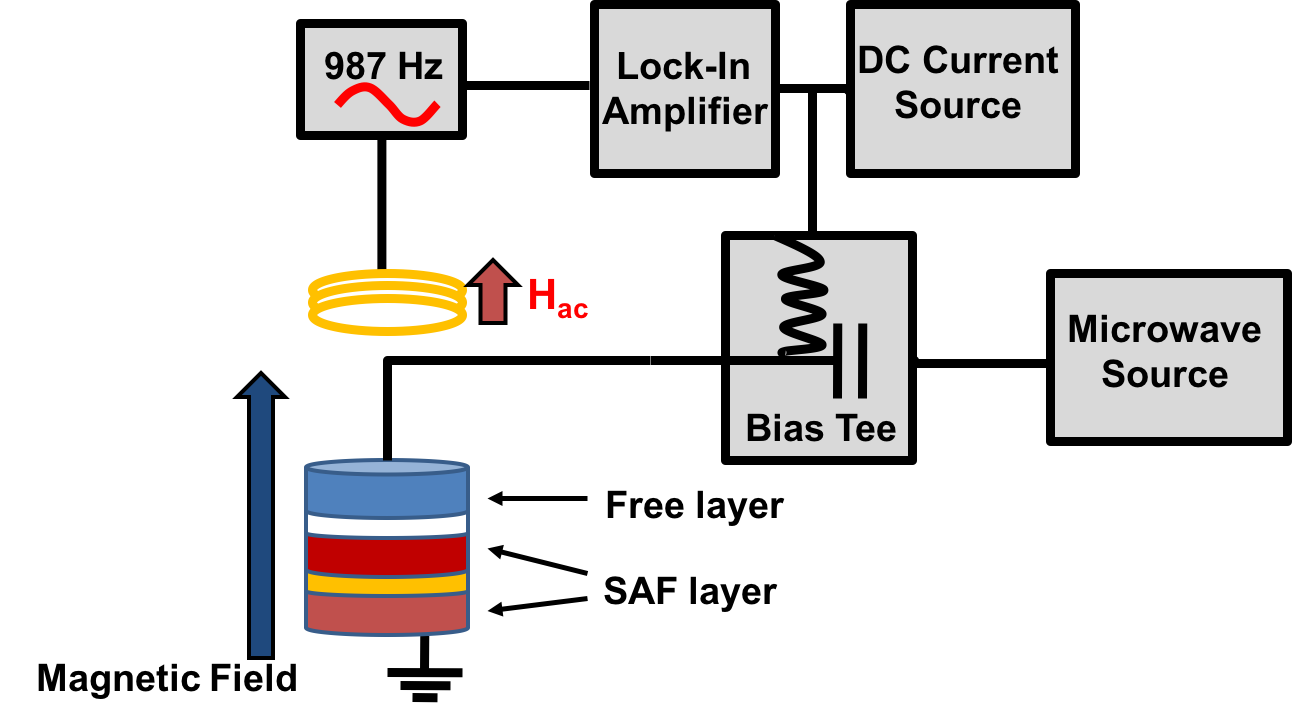
\includegraphics[width=0.8\textwidth]{fig/FieldMod/set_up.png}
    \caption{Sketch of our field-modulation set-up.}
    \label{fig:FMR_set_up}
\end{figure}





\begin{figure}[!ht]
\centering
\subfigure{\label{fig:Amp}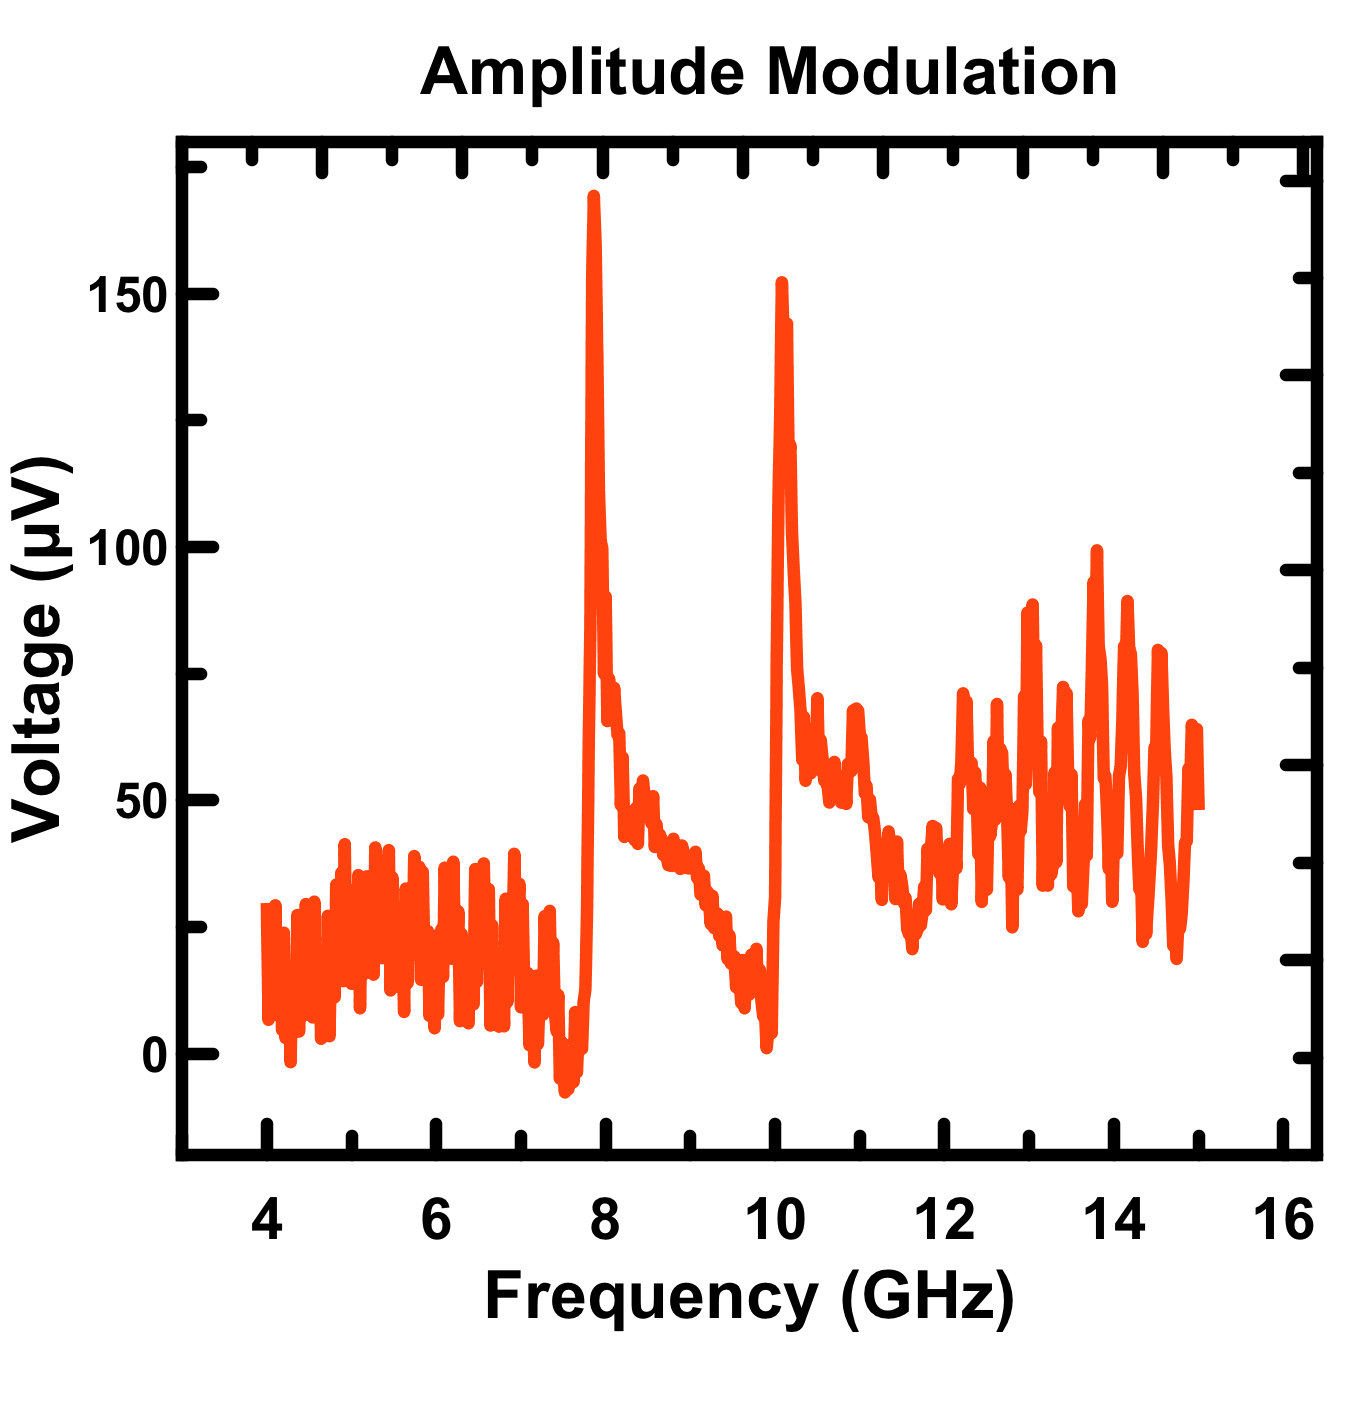
\includegraphics[width=70mm]{fig/FieldMod/AmpMod.png}}
\subfigure{\label{fig:Field}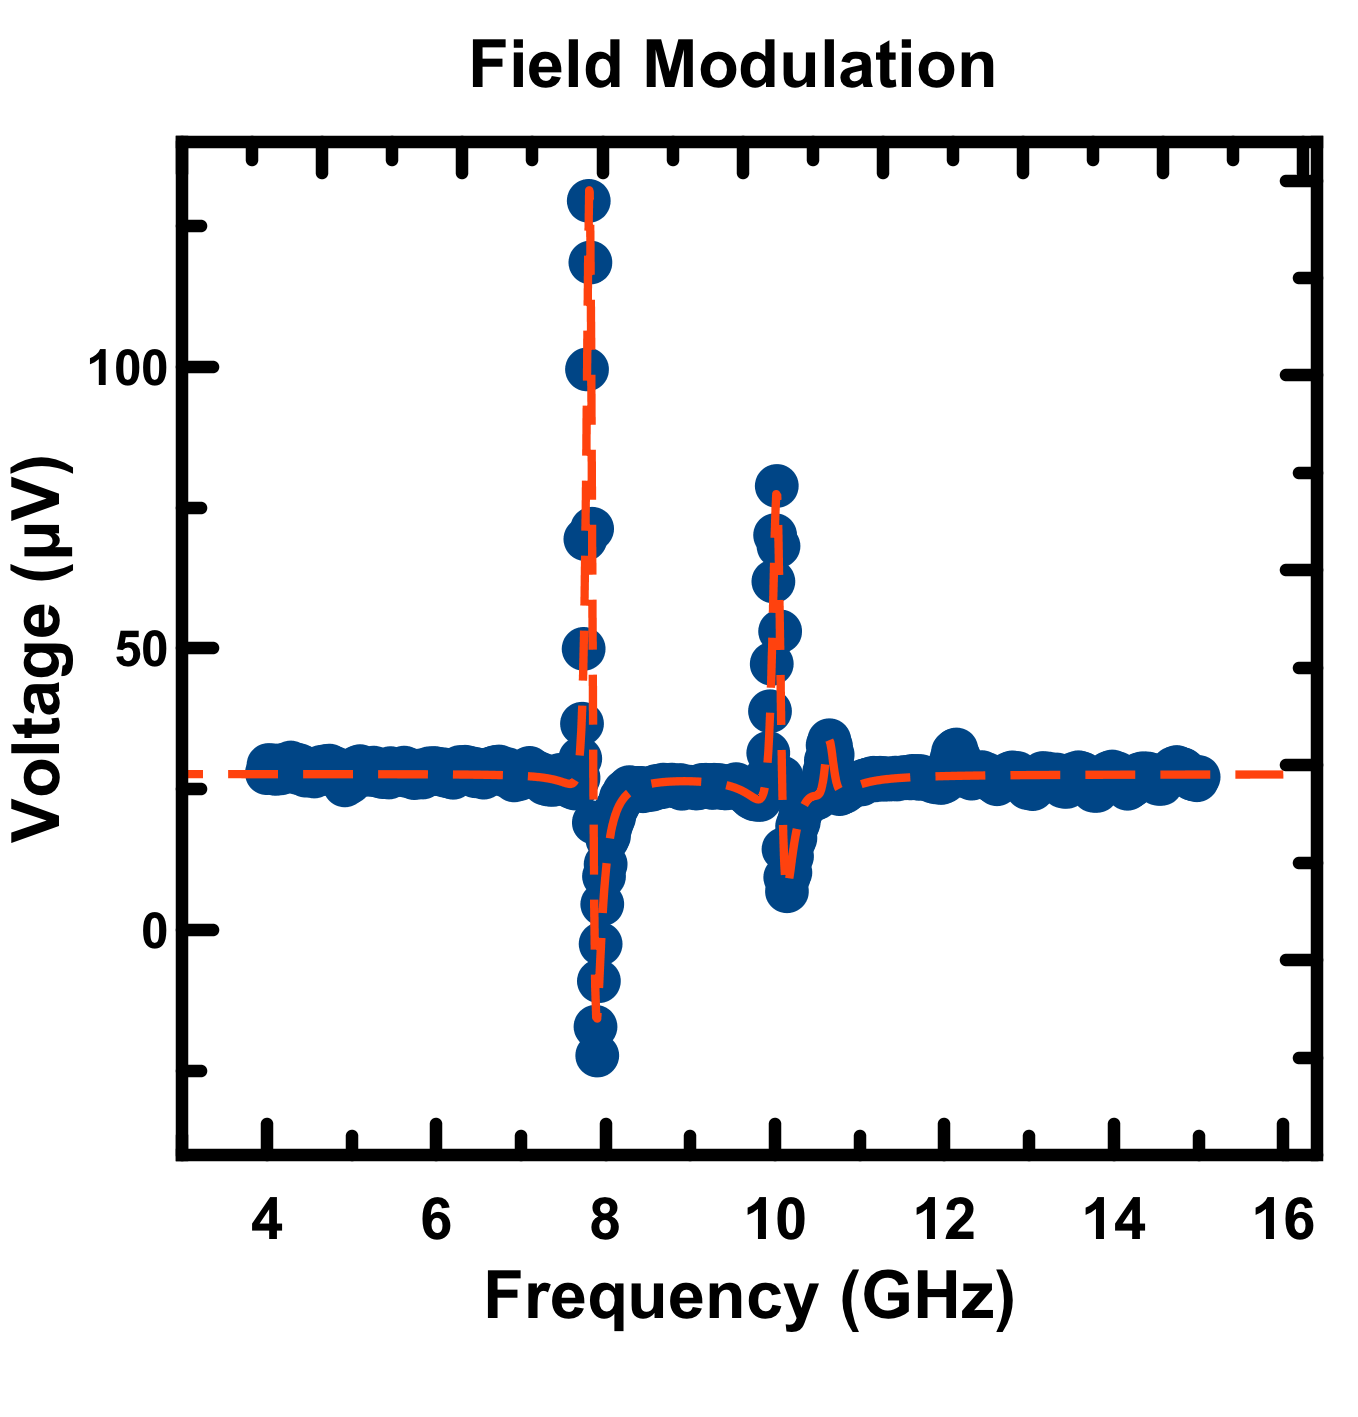
\includegraphics[width=70mm]{fig/FieldMod/FieldMod.png}}
\caption{(a) Typical ST-FMR spectrum taken with conventional amplitude modulation.(b) ST-FMR spectrum taken with field modulation at the same sample.}
\end{figure}





To solve this problem, We make ST-FMR measurement with field modulation technique\cite{FieldMod}. A modulation coil is placed just above the sample as shown in Fig.\ref{fig:FMR_set_up}. We then apply kHz-range sinusodal current of a few Amperes in the coil and generate a few Oersteds alternating magnetic field. The modulation field from the coil is perpendicular to the nanopillar. A continuous microwave current is applied to the sample via a bias tee, and a rectified voltage generated by the sample is measured by a lock-in amplifier at the field modulation frequency. In this case, by sweeping the driving frequency, any non-magnetic background noise would be eliminated. Fig.\ref{fig:Field} shows a typical field-modulation spectrum taken at the same sample comparing with Fig.\ref{fig:Amp}(a). Now we have a much better flat baseline and the standing wave is greatly reduced from the signal.


\begin{figure}[!ht]
\centering
\subfigure{\label{fig:MR}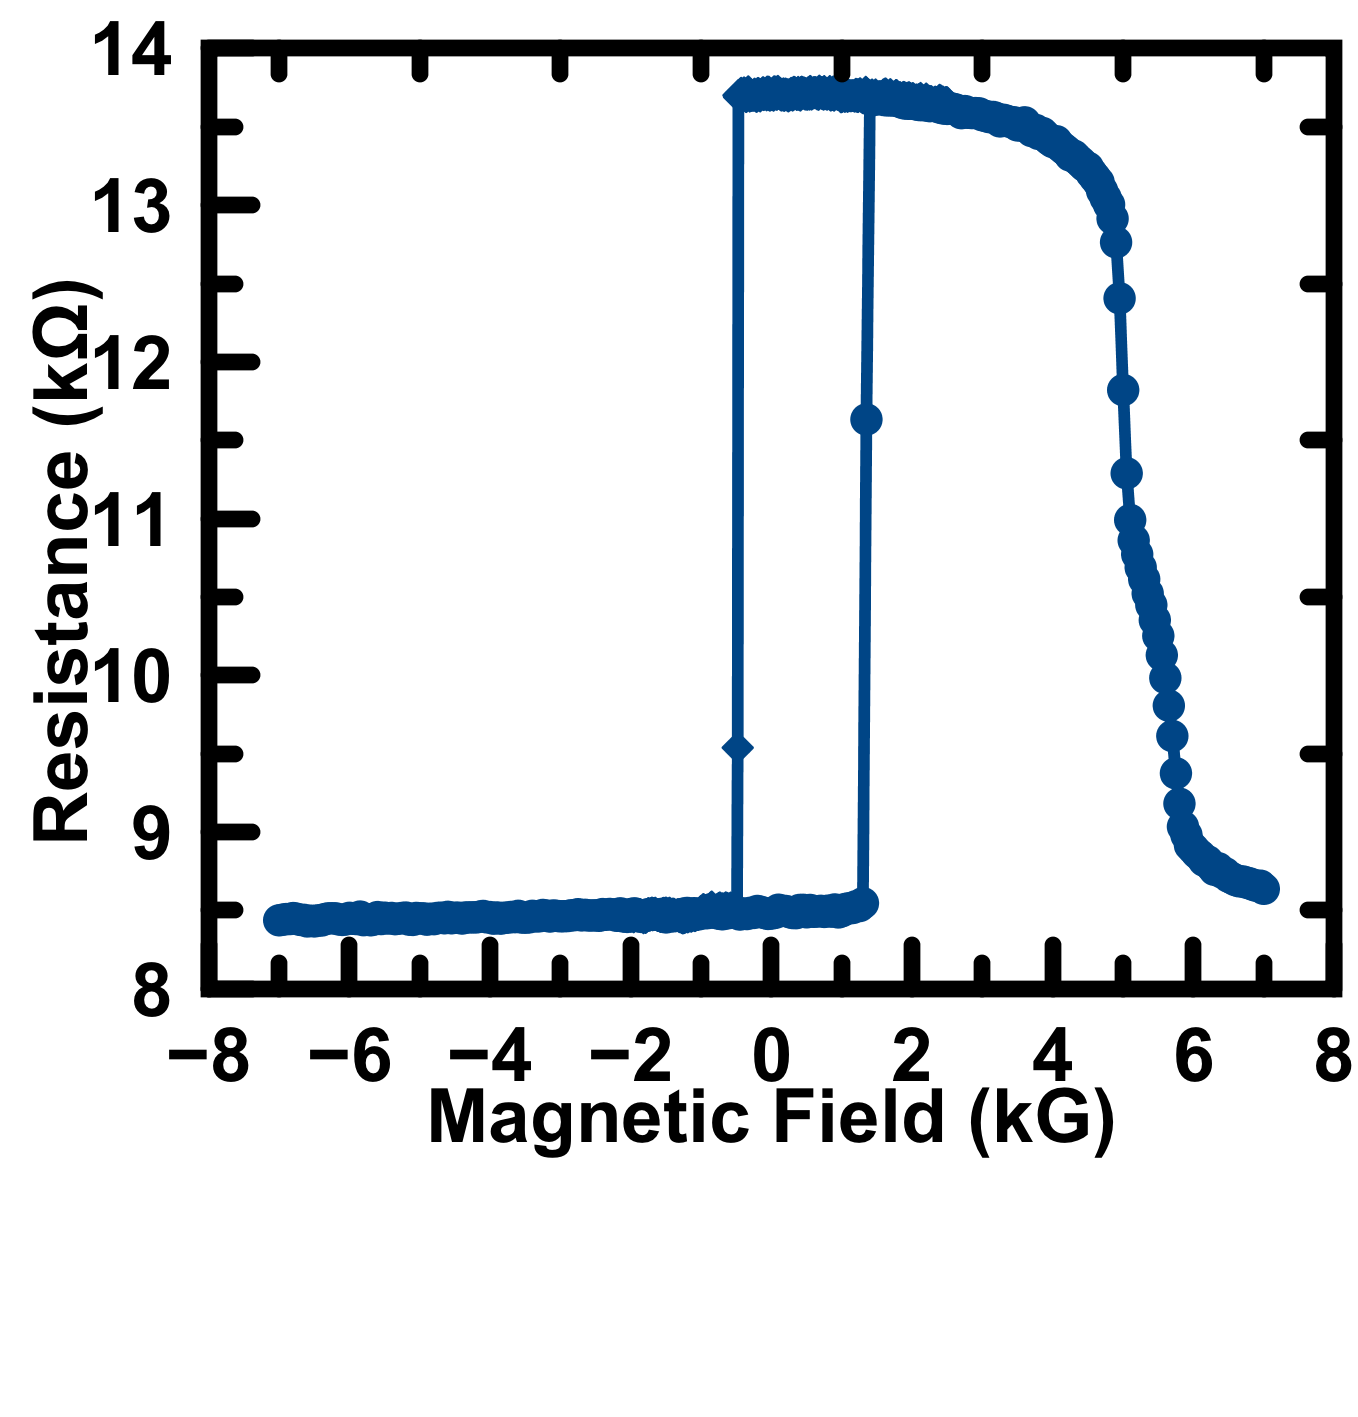
\includegraphics[width=70mm]{fig/FieldMod/MR.png}}
\subfigure{\label{fig:Spectrum}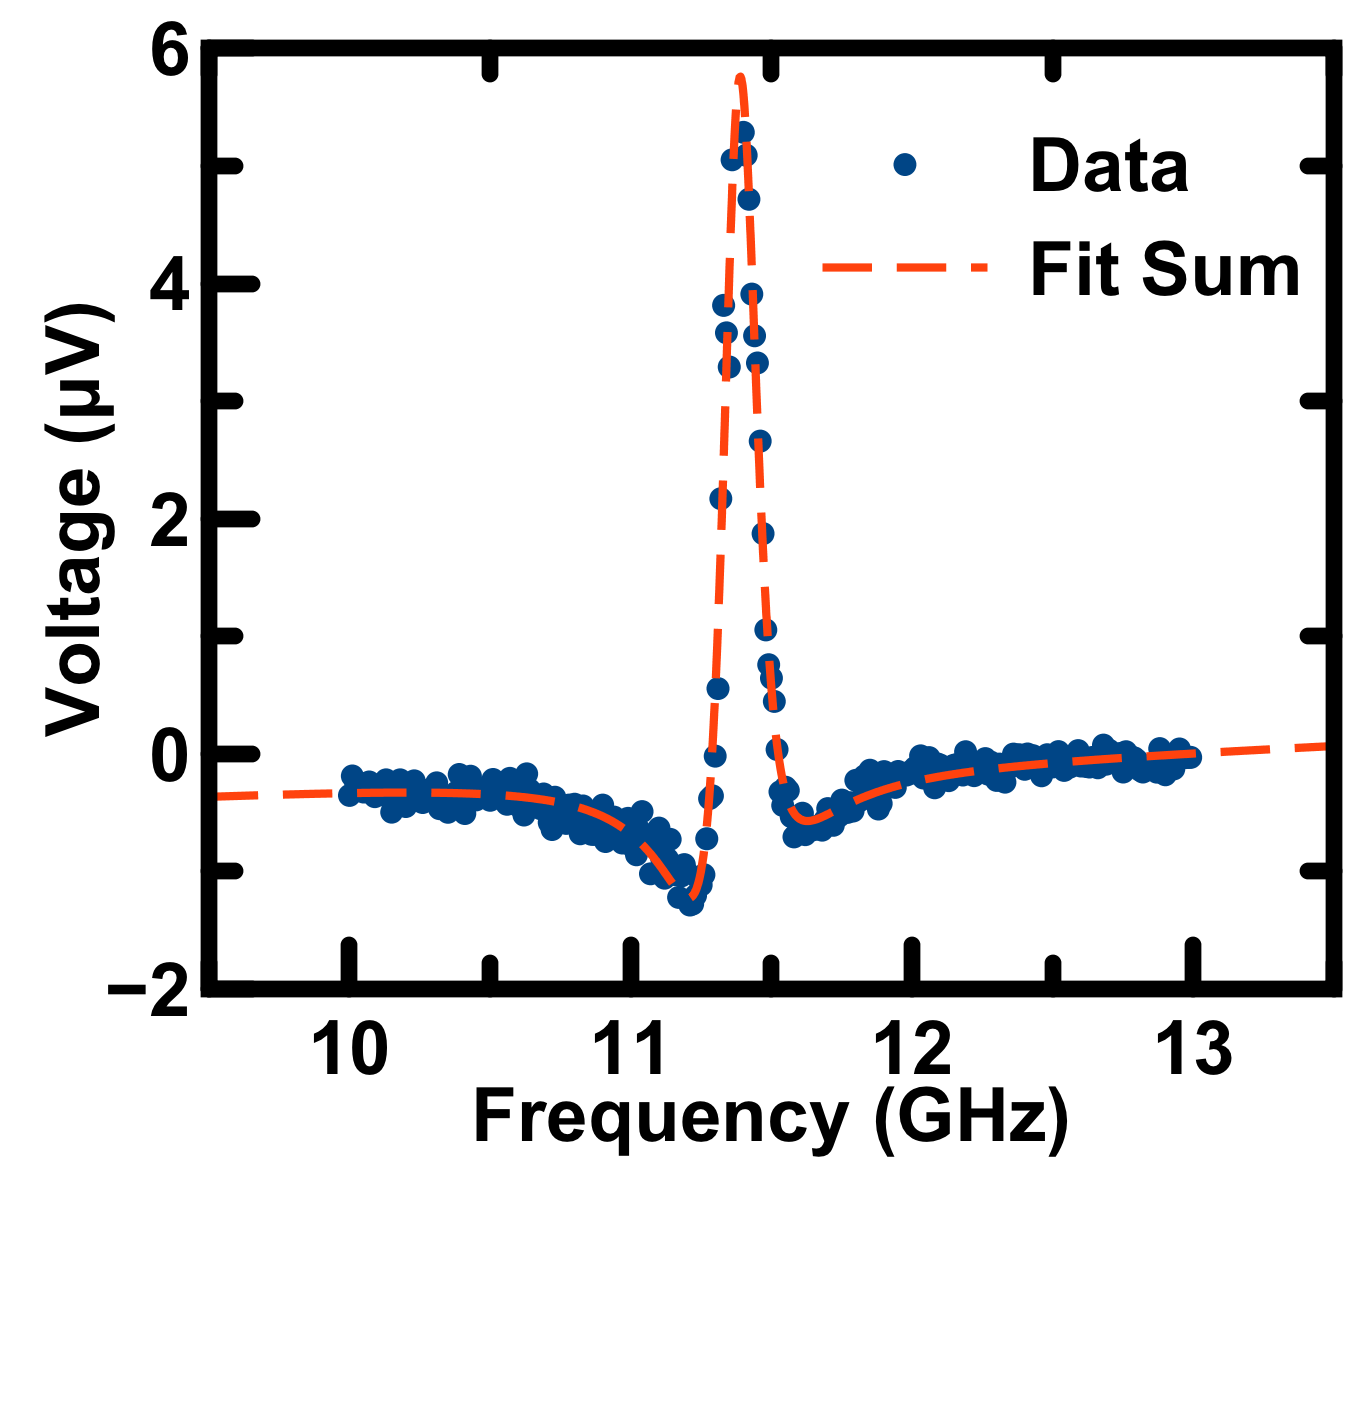
\includegraphics[width=70mm]{fig/FieldMod/Spectrum.png}}

\caption{(a)Magneto-resistance plot of the sample studied. SAFTop layer start to flop around 4.5kG. (b)Blue dot:Typical ST-FMR spectrum with only lowest-frequency mode. Red dash line: Fitted curve to extract resonance frequency and linewidth.}
\end{figure}

The MTJ nanopillar we have measured has a lateral size of 65*30nm with a stadium shape: approximately half-circular on both ends of a rectangular. The main functional layers structure of our sample are SAFBottom(1.67)/SAF spacer(0.41)/SAFTop(1.1)MgO(0.8)FreeLayer(2.4) multilayer(thickness in nm). Fig.\ref{fig:MR} shows the magneto-resistance plot with magnetic field applied perpendicular to the sample. Around 4.5kG, the resistance of the MTJ start to decrease and eventually switch back to low-resistance parallel state. This is due to the flopping of SAFTop layer\cite{Spinflop}. We identify 4.5kG to be the breakdown field and will use it for later discussion.Fig.\ref{fig:Spectrum} shows the ST-FMR spectrum focusing on the lowest-frequency mode. We are now going to derive the mathematical equation to extract resonance frequency and linewidth from the curve.



\section{Gilbert Damping Evaluation}

As we discussed in the previous chapter, the line shape $V_{mix}(f)$  without field modulation is a sum of symmetric $S(f)$ and antisymmetric $A(f)$ Lorentzians $V_{mix}(f) = V_{s}S(f) + V_{a}A(f)$, where $S(f) = \frac{1}{1+(f-f_{r})^{2}/ \sigma_{r}^{2}}$, $A(f) = \frac{(f-f_{r})/\sigma_{r}}{1+(f-f_{r})^{2}/ \sigma_{r}^{2}}$, $f_{r}$ is the resonance frequency and $\sigma_{r}$ is the linewidth. When the modulation field is small, the RMS voltage signal  $\tilde{V}_{mix}(f)$ measured by the lock-in amplifier is proportional to the first derivative of the rectified voltage  $V_{mix}(f)$ with respect to the modulated variable-the external magnetic field $B$.


\begin{equation}
\begin{aligned}
  \tilde{V}_{mix}(f) = & B_{m}\frac{dV_{mix}(f)}{dB} = B_{m}[\frac{dV_{s}}{dB}S(f) + \frac{dV_{s}}{dB}A(f) \\ 
  & + \frac{1}{\sigma_{r}}\frac{d\sigma_r}{dB} 
  \times (2 V_{s} A^{2}(f) + V_{a}[2A^{3}(f)/S(f) - A(f)]) \\
 & + \frac{1}{\sigma_r}\frac{df_{r}}{dB}(2V_{s}S(f)A(f) + V_{a}[A^{2}(f) - S^{2}(f)])]  
\end{aligned}
\end{equation}

Here $B_{m}$ is the RMS amplitude of the modulation field, and the last term proportional to $df_{r}/dB$ is usually dominant. If $V_{s}$ and $V_{a}$ are weak functions of magnetic field then the symmetric part of $\tilde{V}_{mix}(f)$ is proportional to $V_{a}$ and the anti symmetric part is proportional to $V_{f}$.


\begin{figure}[!ht]
\centering
\subfigure{\label{fig:Free}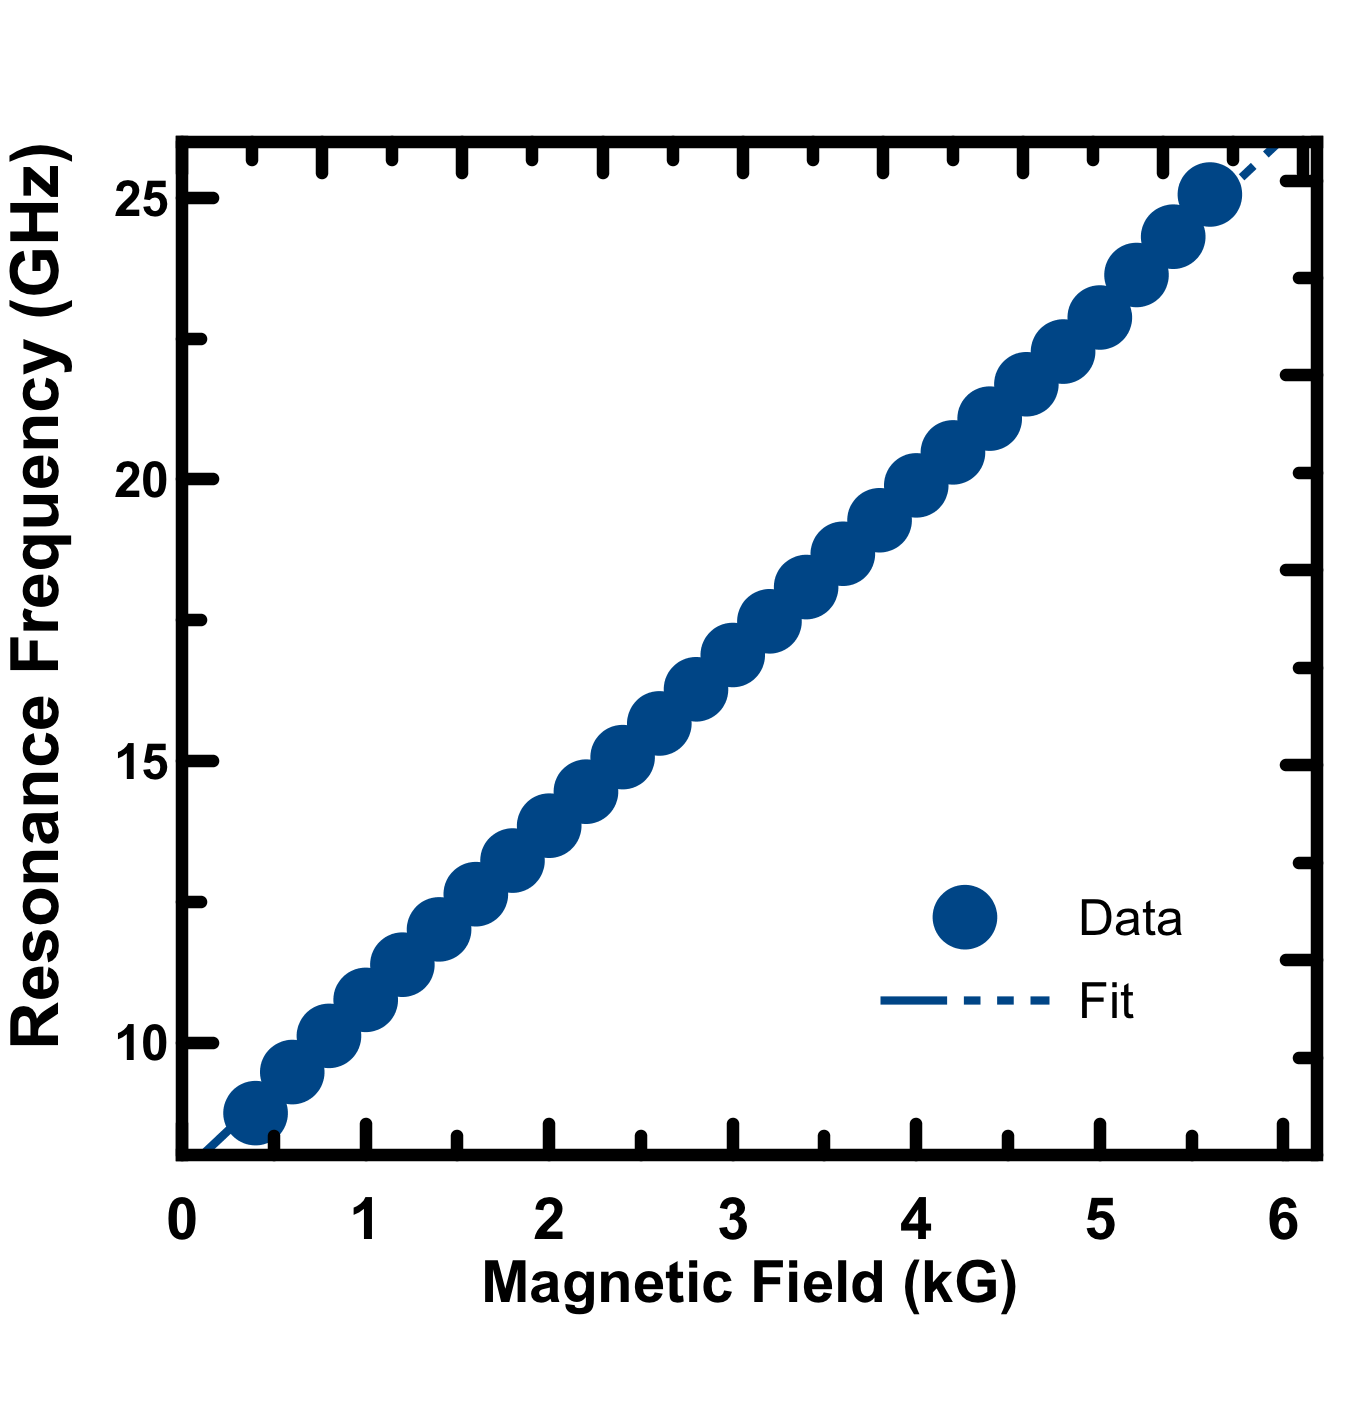
\includegraphics[width=75mm]{fig/FieldMod/Res_Field.png}}
\subfigure{\label{fig:LW}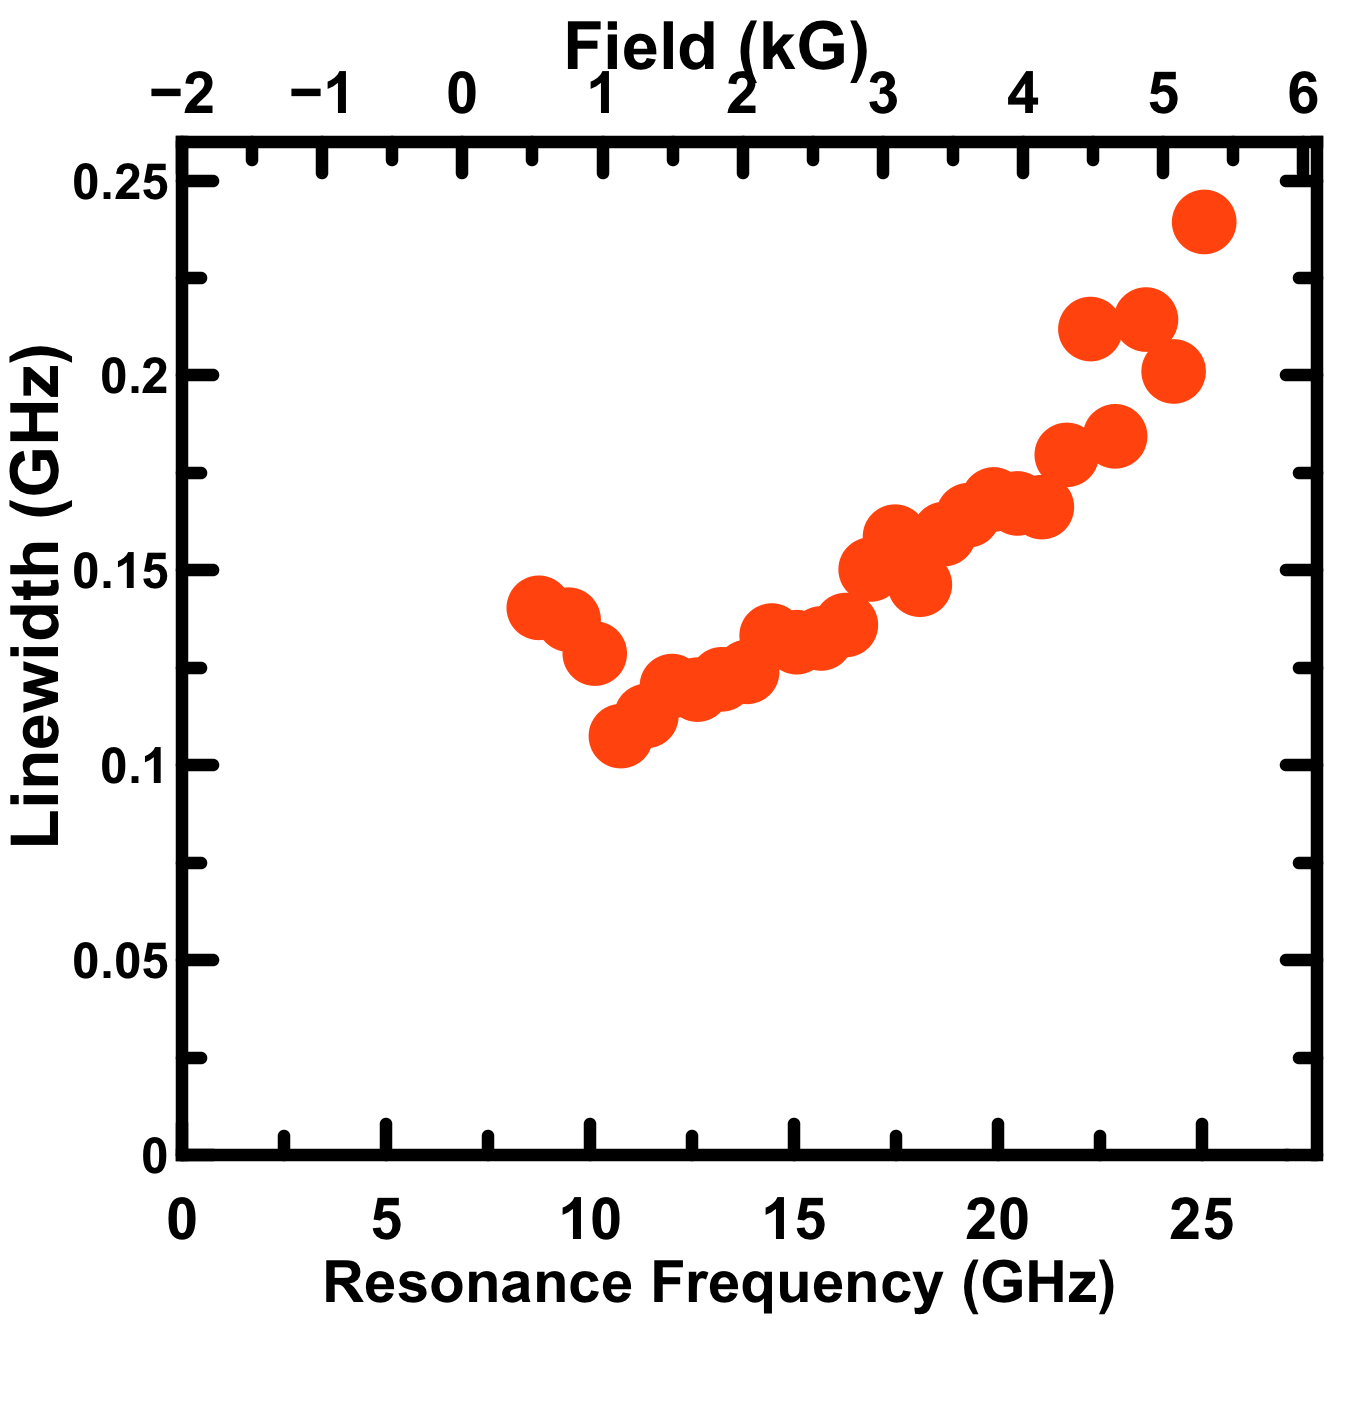
\includegraphics[width=75mm]{fig/FieldMod/Original_LW.png}}
\caption{(a) Fitted resonance frequency plotted against external magnetic field (b)Fitted linewidth plotted as a function of resonance frequency.}
\end{figure}

Fig.\ref{fig:Free} shows the fitted resonance frequency of the quasi-uniform modes respect to the external magnetic field. As we expect from Kittel equation, there is a good linear relation. Making an easy axis approximation, the Kittle equation is 
\begin{equation}
f = \gamma(H_{k} \pm |H_{dip}| + H_{ext})
\end{equation}
Here $H_{dip}$ is the center of hysteresis loop and $H_{ext}$ is the external magnetic field. The quasi-uniform mode frequency at zero field gives magnetic anisotropy field of the free layer ($H_{k}$ = 2.5 kG). 

Next we try to fit for the damping parameter. Precision measurements of the spectral linewidth of the quasi-uniform mode required some improvements of our ST-FMR setup. We found that standing waves in the microwave measurement circuit can introduce significant errors into the measured line width. In order to alleviate the standing wave problem, we introduced a significant length (1.5 – 2 meters) of a microwave cable between the sample and the bias tee used in the ST-FMR setup. This additional length acted as a microwave attenuator that does not generate significant signal reflection (adiabatic absorptive attenuator). Fig\ref{fig:cable} illustrates the degree of improvement of the ST-FMR signal quality offered by the cable attenuator – the spectral peak splitting artifact is completely eliminated and reliable measurements of the spectral linewidth become possible.

\begin{figure}[!ht]
  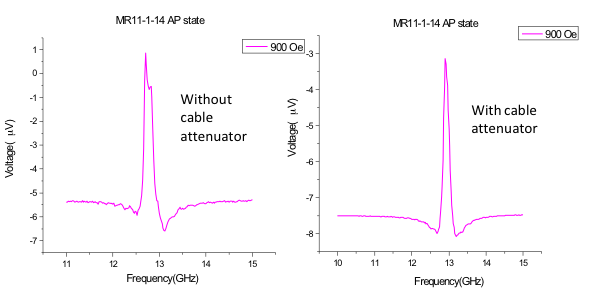
\includegraphics[width=0.8\textwidth]{fig/FieldMod/Improve-measure.png}
  \centering
  \caption{ST-FMR spectrum measured without a long attenuating cable attached to the sample (left) is significantly distorted by standing waves in the microwave circuit. (right) The same spectrum measured with a long attenuating cable eliminates the standing wave artifacts. }
  \label{fig:cable}
\end{figure}






Previous work has been shown that Gilbert damping parameter can be determined from the linewidth from the FMR signal\cite{Bias}. Fig.\ref{fig:LW} shows the linewidth plotted as a function of resonance frequency. We would expect to observe a linear relation if only considering Gilbert damping contribution. From our data,however,we can observe obvious two regions which deviate from a simple linear fitting. Firstly, at low frequency around 10GHz, the linewidth was clearly broadened and was larger than other region. Secondly, at higher frequency above 20GHz, the linewidth has more noise in terms of relative fluctuations. Moreover, if we try to fit the linewidth data and extrapolate to zero frequency, we found there is a large non-zero intercept. It is not clear whether this non-zero intercept is due to some inhomogeneous broadening in our sample or some other mechanism. There exist different mechanism responsible for possible linewidth broadening\cite{3-Magon}.

To fully understand the magnetic dynamics excited in the magnetic tunnel junctions, we make the full ST-FMR measurement and shows the 2D contour plot of the results in Fig.\ref{fig:2D}. At lower magnetic field(0~2kG), we can mainly observe three free layer modes. These three modes are parallel to each other and the lowest frequency Q mode is the quasi-uniform mode, which has been used to determine the anisotropy constant. Two higher order mode labeled as F1 and F2 are distinct from this 2D contour plot although they are hard to distinguish from single spectrum.
Starting from 2kG, at lower frequency, there is another mode appearing in the contour plot. This mode,labeled as S mode, has a different dispersion relation: the resonance frequency decreases with increasing magnetic field. This mode can be identified as acoustic mode generating from the SAF layer. The important feature here is that, if we extrapolate the S mode into lower magnetic field, the S mode will be coupled with Q mode around 10GHz at zero field.  

\begin{figure}[!ht]
  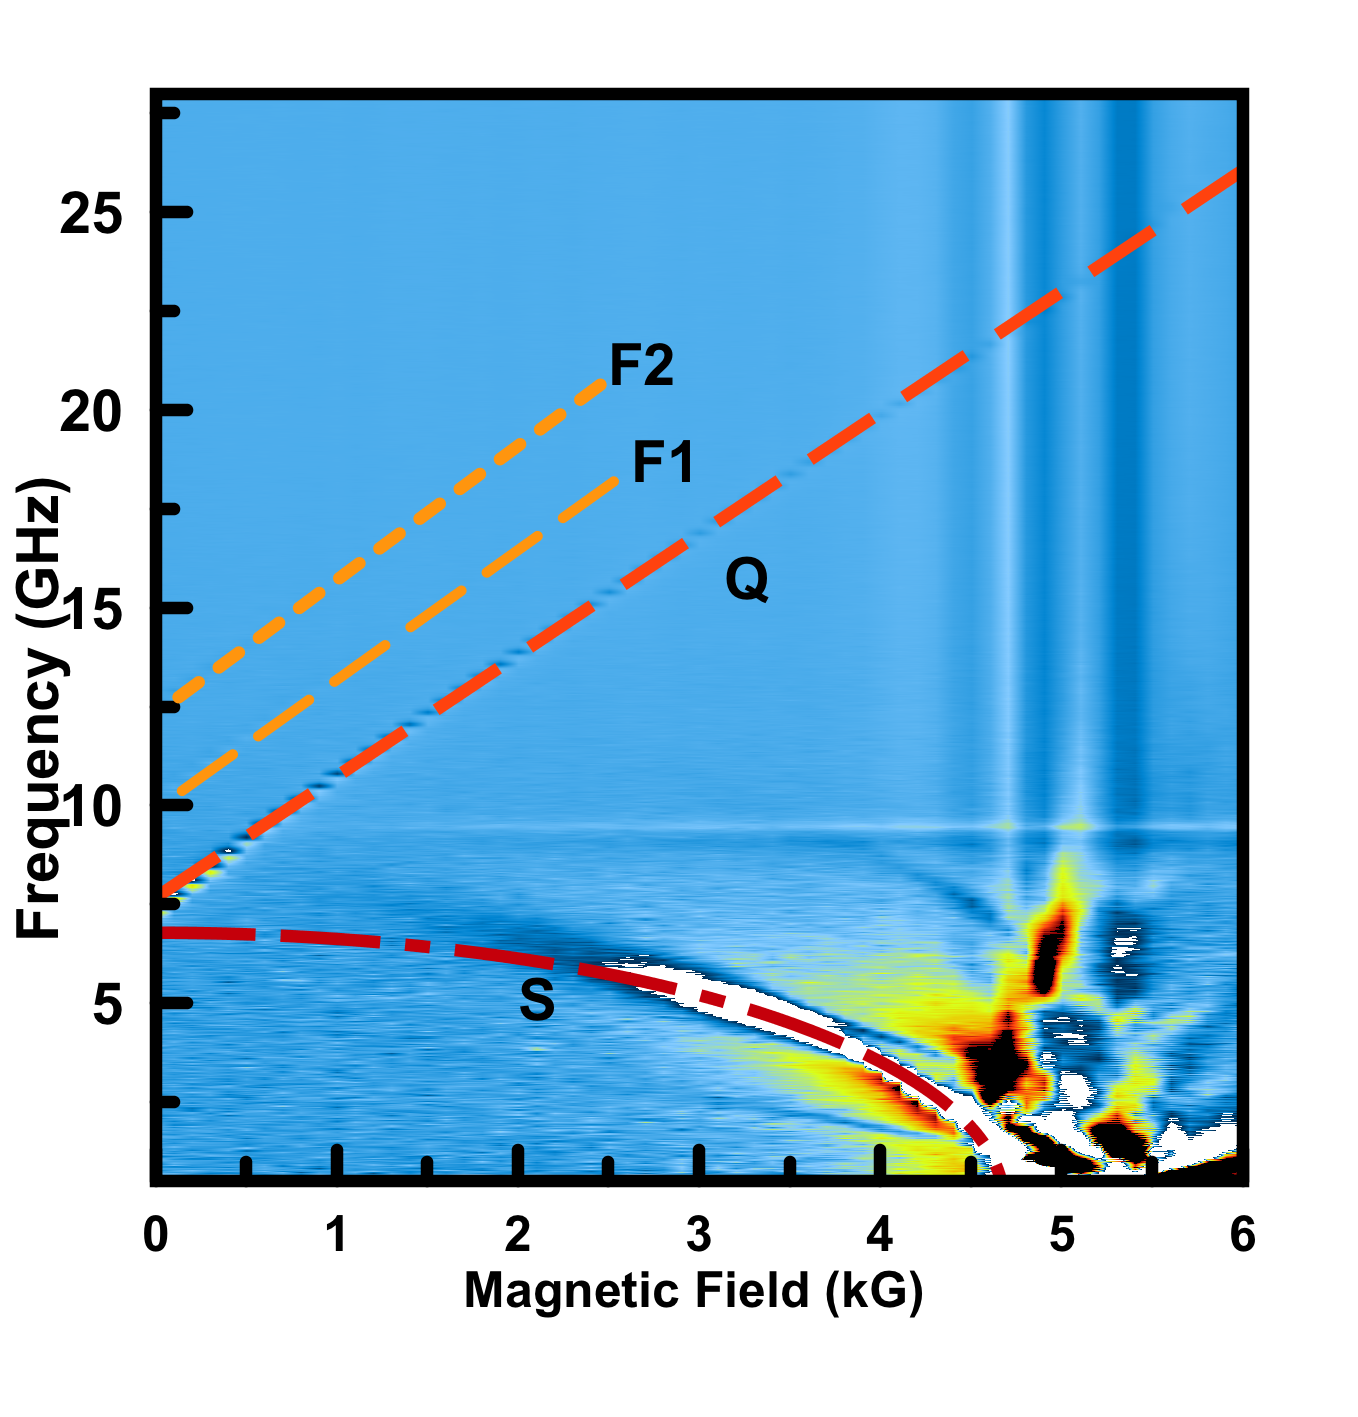
\includegraphics[width=0.8\textwidth]{fig/FieldMod/contour.png}
  \centering
  \caption{ST-FMR spectra measured as a function of out-of-plane magnetic field. Q labels the quasi-uniform mode of the free layer while F2 and F3 are the higher order spin wave modes of the free layer. S labels the acoustic SAF mode. }
  \label{fig:2D}
\end{figure}


When we have the resonant coupling between these two modes, the linewidth would be broadened by this resonant coupling mechanism. This is exactly what we have found from Fig.\ref{fig:2D} in the lower frequency region.

In the 2D contour plot, around 4kG magnetic field, as we can see from Fig.\ref{fig:d}, the SAF layer becomes unstable and enter the spin-flop region. In this region, because of unstable SAF layer, the stray field from SAF layer acting on the free layer is also very unstable and produce large magnetic noise during the ST-FMR measurement. As a result, we find there are more fluctuations in the linewidth data as we see from Fig.\ref{fig:LW} around 20GHz.

As we have learned from the 2D contour plot, in order to reliably fit for the damping parameter in the free layer, we need to first exclude the resonant coupling region in the lower frequency, in which the linewidth was broadened by the interaction between free and SAF layer. We also need to avoid the high frequency region. In Fig.\ref{fig:LW_FIT} we only include the linewidth data from 10GHz to 20GHz and determine the Gilbert damping to be 0.007 from the slope.
 
\begin{figure}[h]
  \centering
  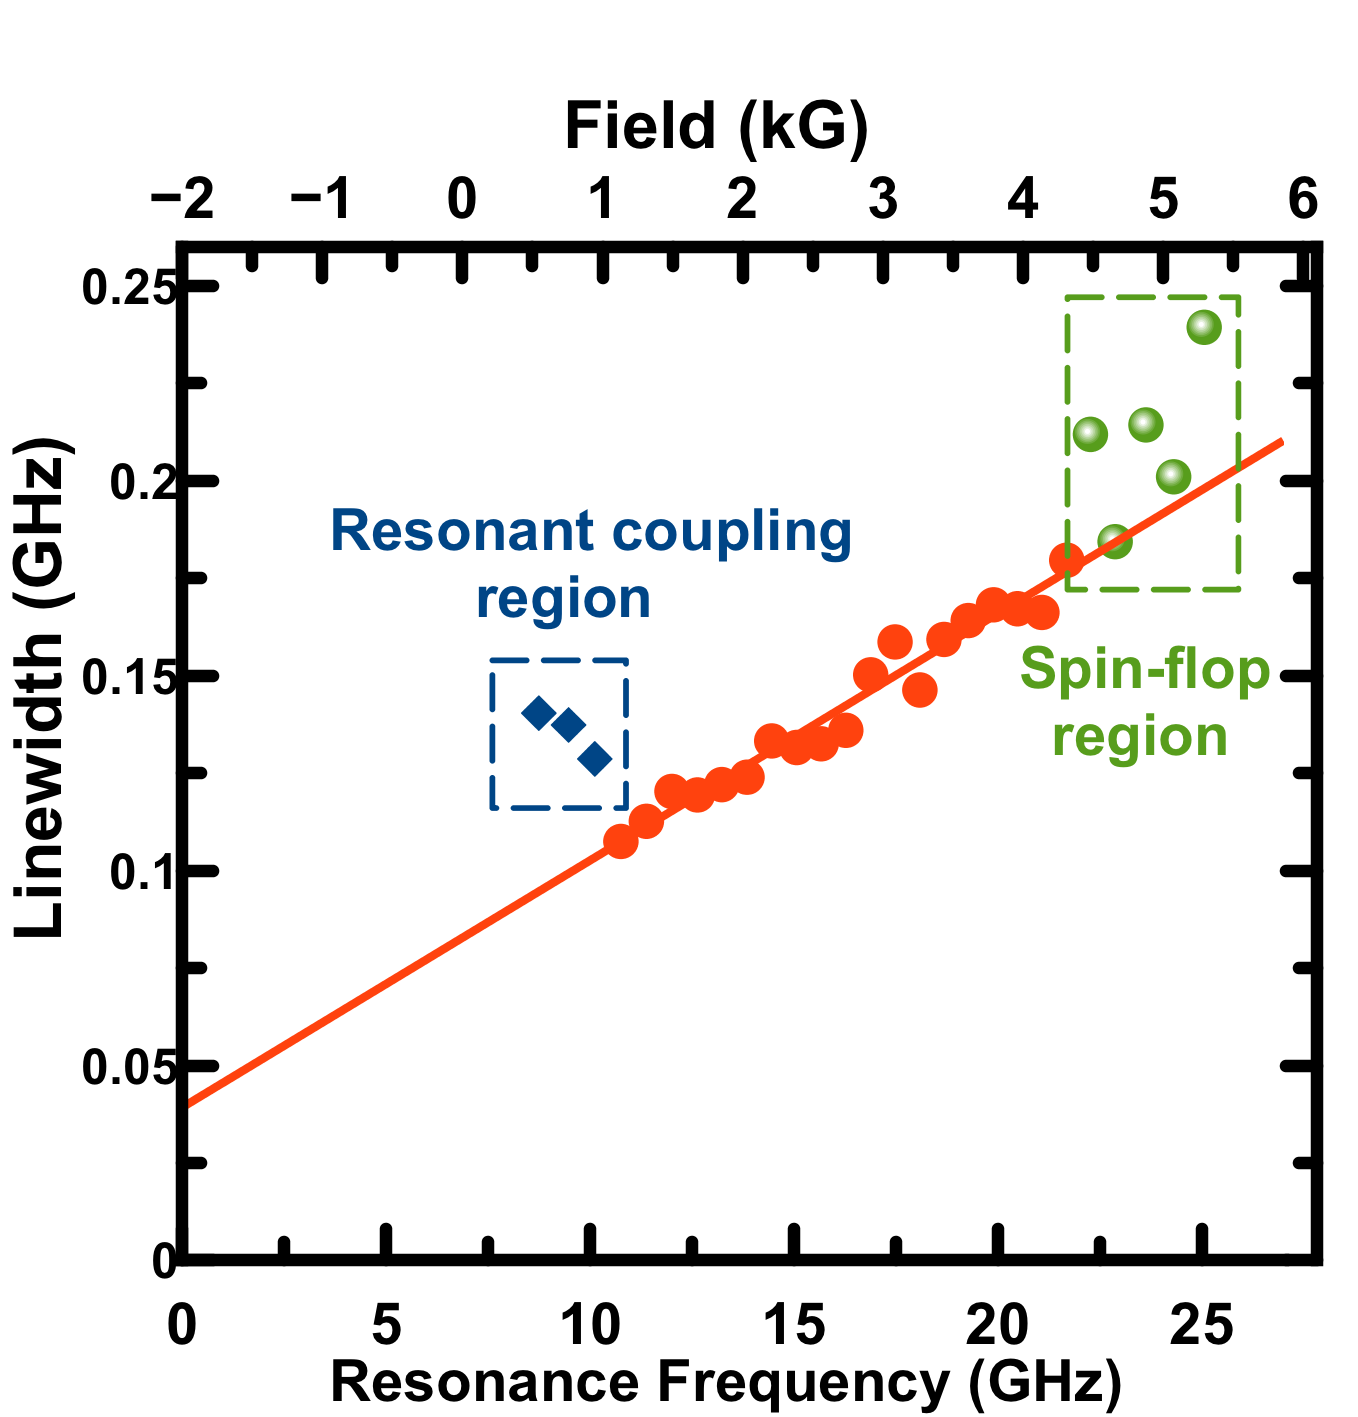
\includegraphics[width=0.8\textwidth]{fig/FieldMod/LW_PLOT.png}
  \caption{Spectral linewidth of the free layer quasi-uniform mode versus frequency of the mode. Line is the best fit to the data outside of the SAF spin flop and SAF resonant coupling regions.}
  \label{fig:LW_FIT}
\end{figure}

Here the intercept $\Delta f_0$ is linewidth at zero resonance frequency, which is often due to inhomogeneous effects such as the dispersion in effective anisotropy field from the distributions of demagnetization field and stray field\cite{inhom}. From the fitting of the slope, we obtain a low Gilbert damping value around 0.006, which is consistent with other measured Gilbert damping value for the CoFeB-based free layer in similar work\cite{STFMR_1}. Such a small value of Gilbert damping is essential for lowering critical switching voltage as we previously discussed. The critical switching voltage given by Eq.\ref{eq:criticalV} is 0.85 V. From the intercept at zero resonance frequency, we obtained the intercept $\Delta f_0$ around 0.0392 GHz. We would like to further investigate the non-zero intercept and the inhomogeneity in the free layer of the MTJs by micromagnetic simulations.








\section{Continous wave Micromagnetic Simulations}

To understand the linewidth and nature of non-intercept intercept we observed, we perform continuous wave micromagnetic simulations of magnetization dynamics using OOMMF software\cite{OOMMF}. To fully account the magnetic dynamics in all layers, we employ a three-dimensional with three ferromagnetic layers: free, SAF top and SAF bottom. We use material parameters obtained from independent measurements and/or their accepted literature values. The cell size used is 0.25 nm, which is comparable to the grain size observed in the CoFeB system\cite{grain}. 

\begin{figure}[h]
  \centering
  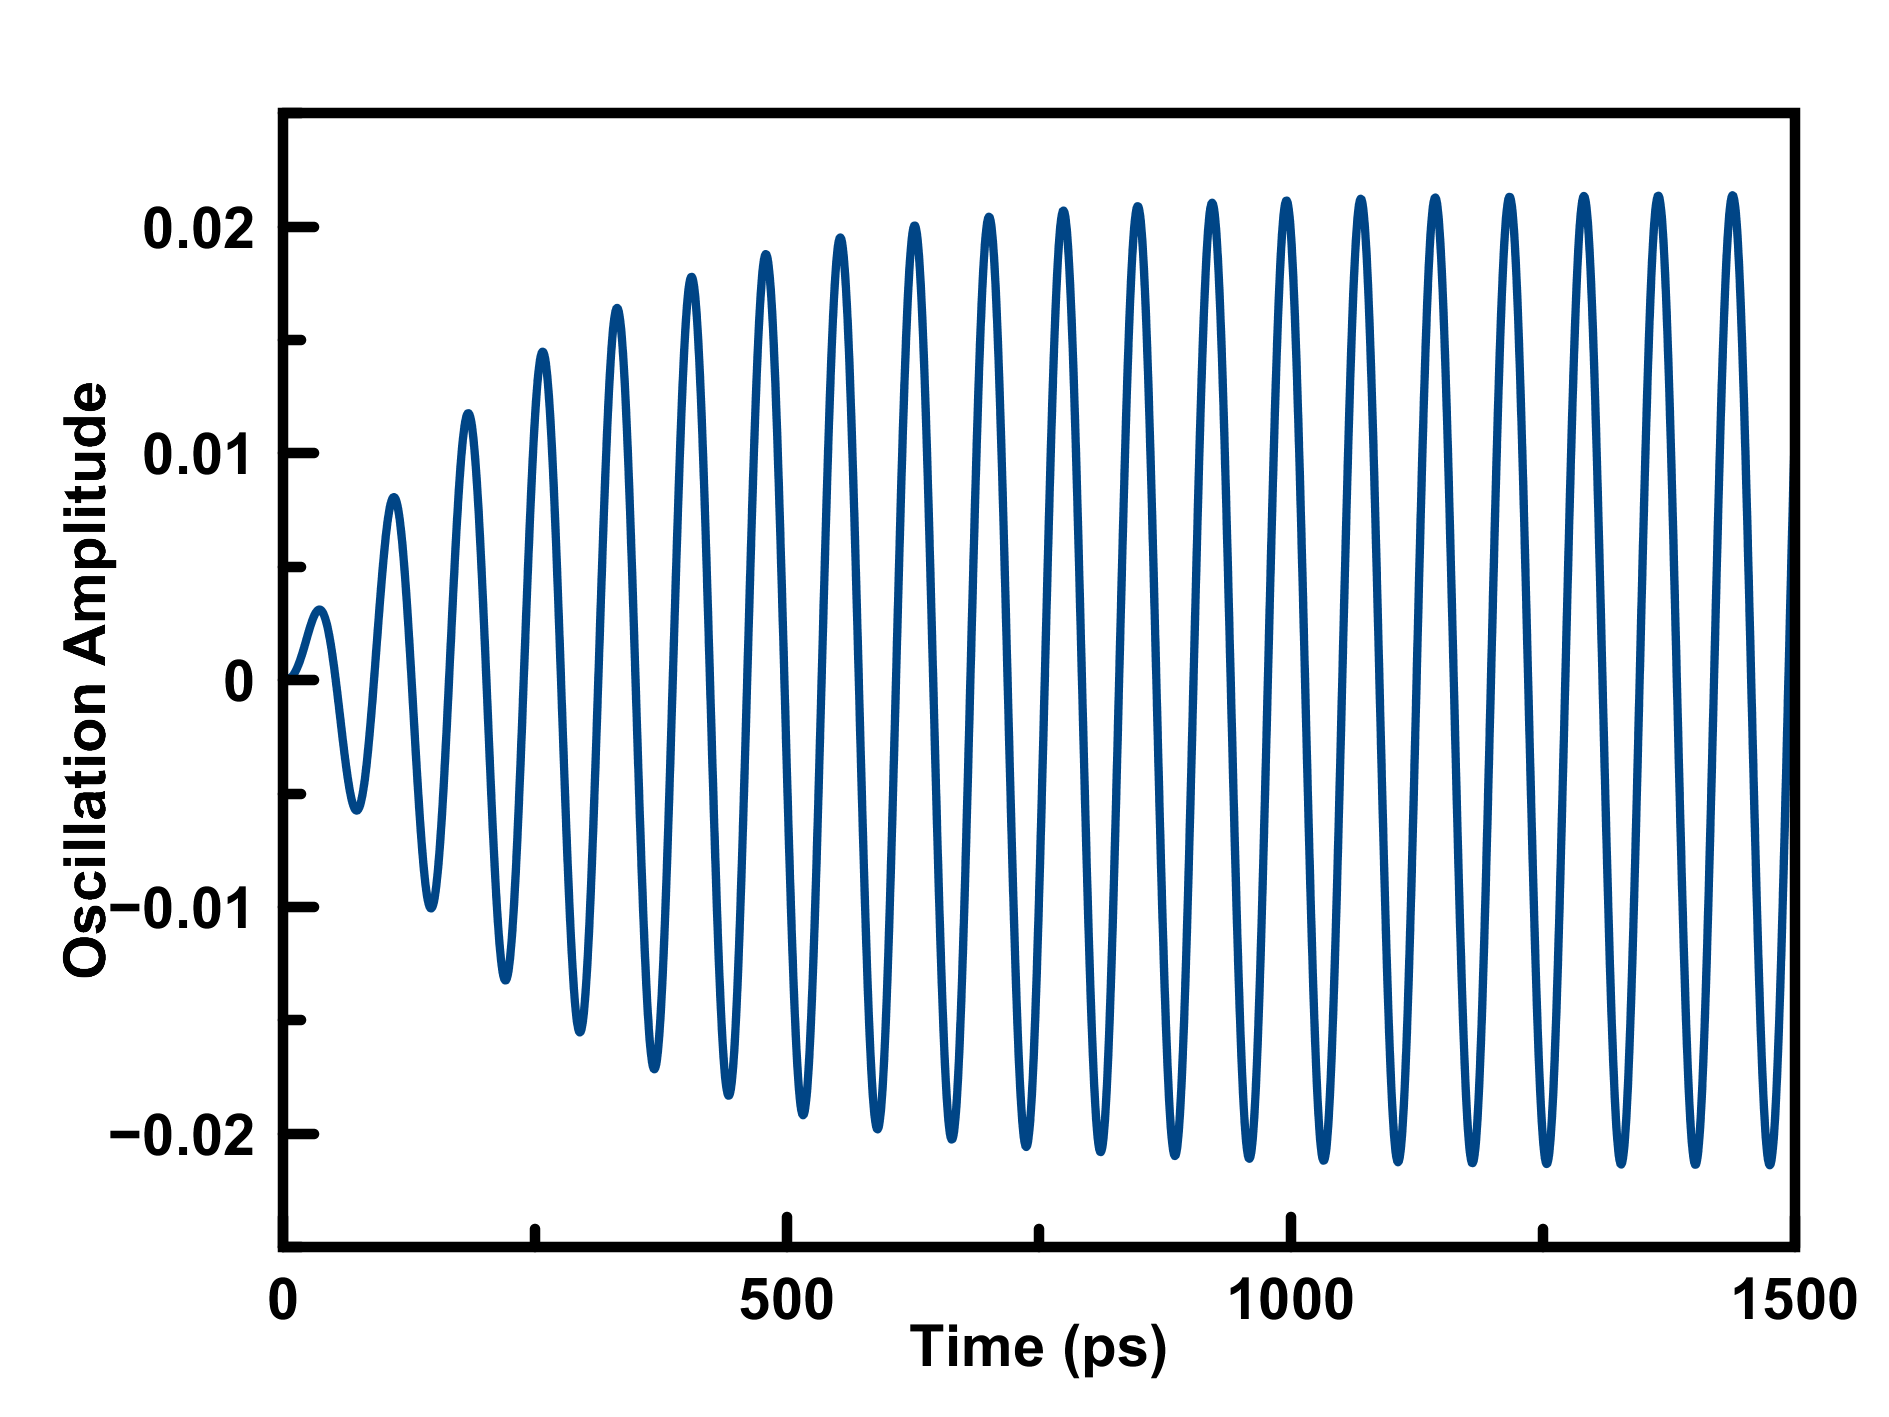
\includegraphics[width=0.6\textwidth]{fig/Time_oscillation.png}
  \caption{Spectral linewidth of the free layer quasi-uniform mode versus frequency of the mode. Line is the best fit to the data outside of the SAF spin flop and SAF resonant coupling regions.}
  \label{fig:timeOscilation}
\end{figure}

In the simulations, the spin wave dynamics is excited by a combined pulse of spin-torque and Oersted field, both resulting from a sine-wave-driven current. During the simulation process, we first relax the system under static magnetic field to reach the ground state. Then the magnetization is excited by sine-wave drive and oscillate with increasing amplitude. After a certain period of transient time, the magnetization will precess steadily and enter dynamic equilibrium. To illustrate this process, we can plot the magnetization as a function of simulation time as shown in Fig.\ref{fig:timeOscilation}. The magnetization first undergoes a period of transient time and then enter a steady oscillations, which yields a certain value of oscillation amplitude and phase. For each driven frequency, we can determine corresponding amplitude of the oscillation at a constant magnetic field. The blue dot from Fig.\ref{fig:Sim_spectrum} show the oscillation amplitude of the in-plane component of magnetization as a function of applied  frequency at 2000 Oe field, which shows a typical Lorentzian curve as expected\cite{Tulapurkar2005}. From the simulation, We can adjust the perpendicular uniaxial anisotropy in order to reproduce the same experimental resonance frequency(7.54 GHz) at zero magnetic fields. The fitted uniaxial anisotropy  is $4.05 \times 10^5 J/ m^3$. Compared with the magnetic anisotropy field we measured from field-modulated ST-FMR methods, we can also calculate the perpendicular uniaxial anisotropy field from the following equation \cite{Ohno2010}

\begin{equation}\label{eq:hk}
H_k = 2 K_u /M_ s - 4 \pi M_s . 
\end{equation}


Here $H_k$ is the effective magnetic anisotropy, $K_u$ is the uniaxial perpendicular magnetic anisotropy and $M_s$ is the saturation magnetization. The PMA calculated from experimental value is $4.73 \times 10^5 J/ m^3$, which has around 15\% deviation from micromagnetic simulated value. This discrepancy in the magnetic anisotropy shows the deviations between the macrospin Kittel equation and the simulated micromagnetic model.  


\begin{figure*}[t]
\centering     
\subfigure{\label{fig:uniform_spectrum}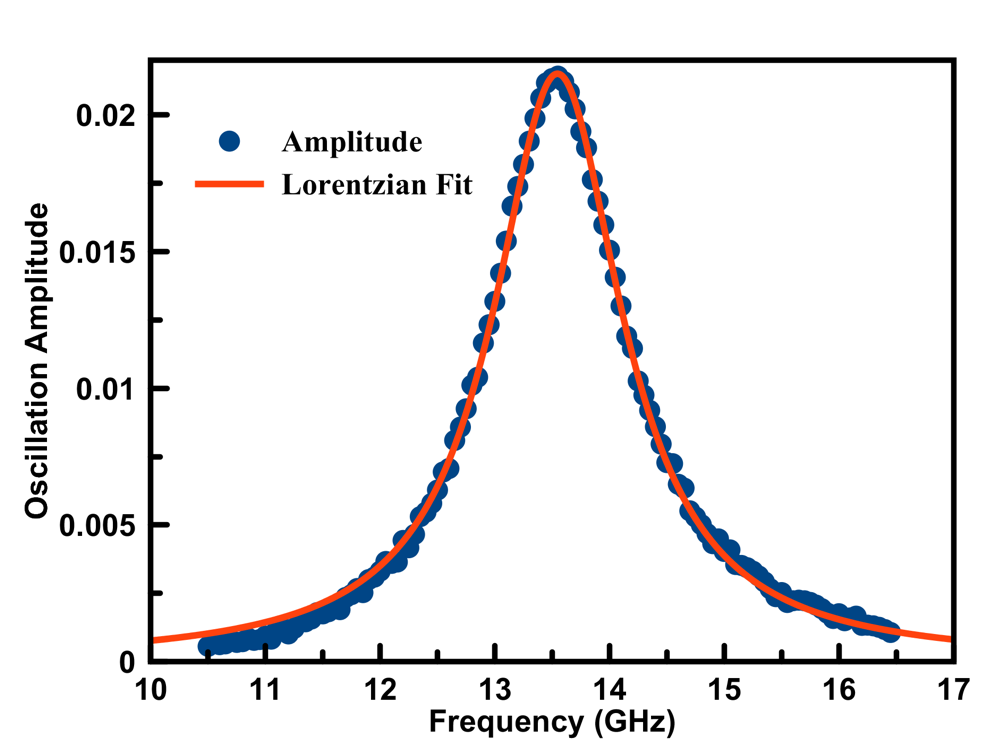
\includegraphics[width=70mm]{fig/CW_sim/uniform_spectrum.png}}
\subfigure{\label{fig:uniform_mode_profile}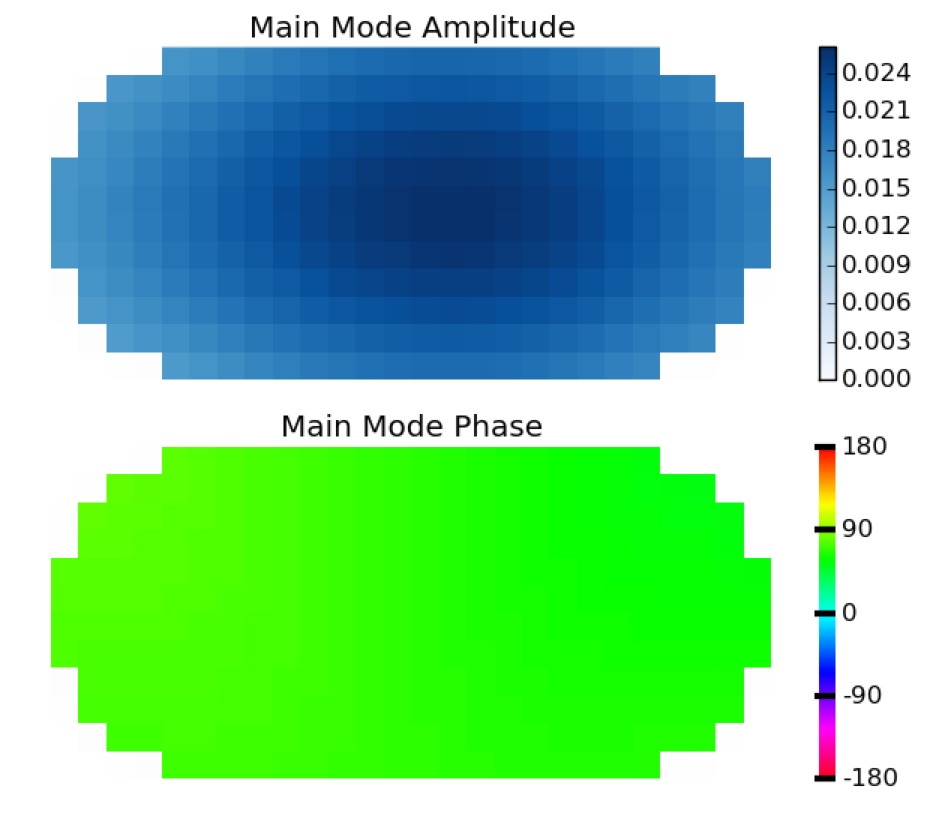
\includegraphics[width=70mm]{fig/CW_sim/mode_profile_1.png}}
\caption{(a)Blue dot: Simulated amplitude versus driven frequency. Red line: Fitted Lorentizan curve. (b)Spatial profile of mode amplitude(Top) and phase(Bottom) of the mode excited in the continuous wave. The amplitude and phase are both uniform across the device, indicating a quasi-uniform eigenmode. }
\end{figure*}


Let us now focus the simulated linewidth from this continuous wave simulations. In this type of simulation, we adopt the Gilbert damping value of 0.05 to avoid longer relaxation and simulation time. By simulating the spectrum at the different magnetic field, we can also fit for the resonance frequency and linewidth as we have done experimentally in Fig.\ref{fig:LW}. The blue dot and dashed line in Fig.\ref{fig:uniform_lw} shows such data from this simulation. The fitted  Gilbert damping constant $\alpha$ is 0.05 with an intercept at zero frequency $\Delta f_0$ 0.002, which shows that at this perfectly uniform model, the inhomogeneous broadening should be really weak and the $\Delta f_0$ should be close to zero. We find that this type of finite cell simulation does not introduce a large non-zero intercept at zero frequency as we observed from the experiment.

\begin{figure}[h]
  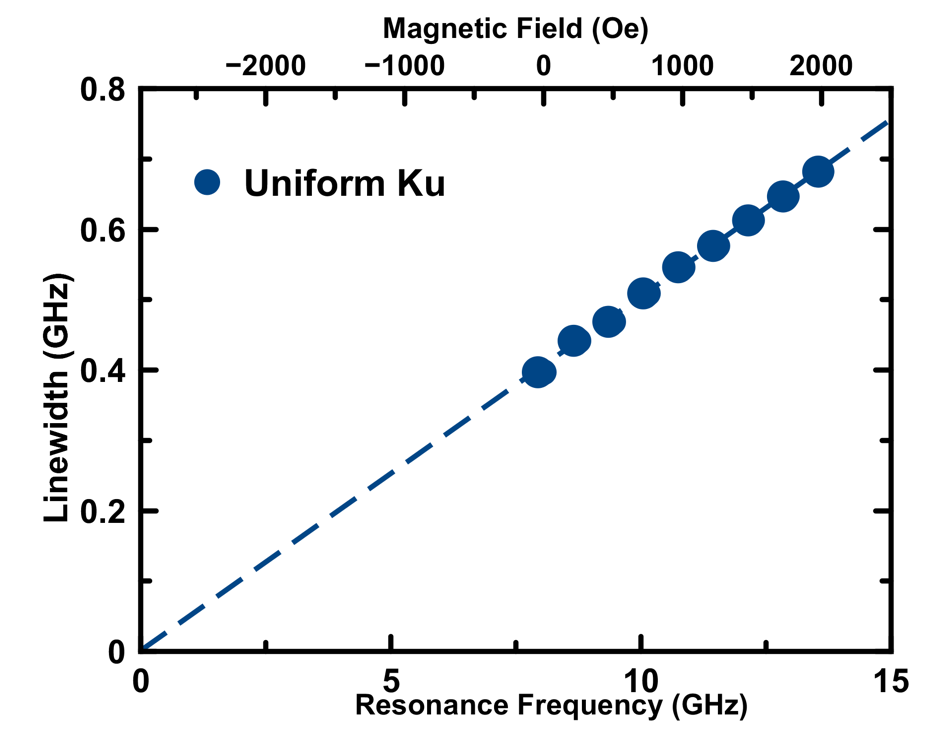
\includegraphics[width=0.6\textwidth]{fig/CW_sim/uniform_LW.png}
  \centering
  \caption{ST-FMR spectra measured as a function of out-of-plane magnetic field. Q labels the quasi-uniform mode of the free layer while F2 and F3 are the higher order spin wave modes of the free layer. S labels the acoustic SAF mode. }
  \label{fig:uniform_lw}
\end{figure}

In the next step of the micromagnetic simulation, we introduce a random anisotropy field that varies spatially. The perpendicular uniaxial anisotropy value at the micromagnetic cell is drawn uniformly from the minimum and the maximum value, which are $3.55 \times 10^5 J/ m^3 $ and  $4.55 \times 10^5 J/ m^3 $ respectively. This variation in the perpendicular uniaxial anisotropy corresponding to the effective magnetic anisotropy to range from in-plane direction 0.1 kG to perpendicular direction 0.21 kG in the simulations(assuming uniform magnetizations across the free layer). We can then repeat the simulation procedure as described above. The red dot and fitted curve at Fig. \ref{fig:random_spectrum} shows the amplitude versus frequency response with this anisotropy fluctuations. Now we still have a Lorentzian curve with some extra noise, which is due to the randomness of anisotropy introduced in the free layer. We can still look at the mode amplitude and phase, as shown in Fig.\ref{fig:random_mode_profile}. Compared with Fig.\ref{fig:uniform_mode_profile} we start to some deviations from uniform excitations, with nodes along the edges. Fig.\ref{fig:Hk_dist} shows the spatial distributions of the random anisotropy across the sample. We can also plot the linewidth as a function of resonance frequency as shown in the green dot in Fig.\ref{fig:CW_lw_summary}. The fitted Gilbert damping value is 0.051 with a intercept -0.0027 GHz. From here we can conclude that only introducing random fluctuations of anisotropy does not reproduce the experimental intercept value.




In the final step of the simulation, we decrease the exchange constant between each grain from 20 pJ/m to  5 pJ/m. We can also plot the linewidth versus frequency as it is shown in the red dot from Fig.\ref{fig:CW_lw_summary}. The slope of this green line gives a Gilbert damping value of 0.04733, which is slightly different from the input damping value. Most importantly, the intercept  at zero frequency $\Delta f_0$ is broadened to  0.043. This value is indeed close to our experimentally determined $\Delta f_0$, 0.0392.  

\begin{figure*}[t]
\centering     
\subfigure{\label{fig:random_spectrum}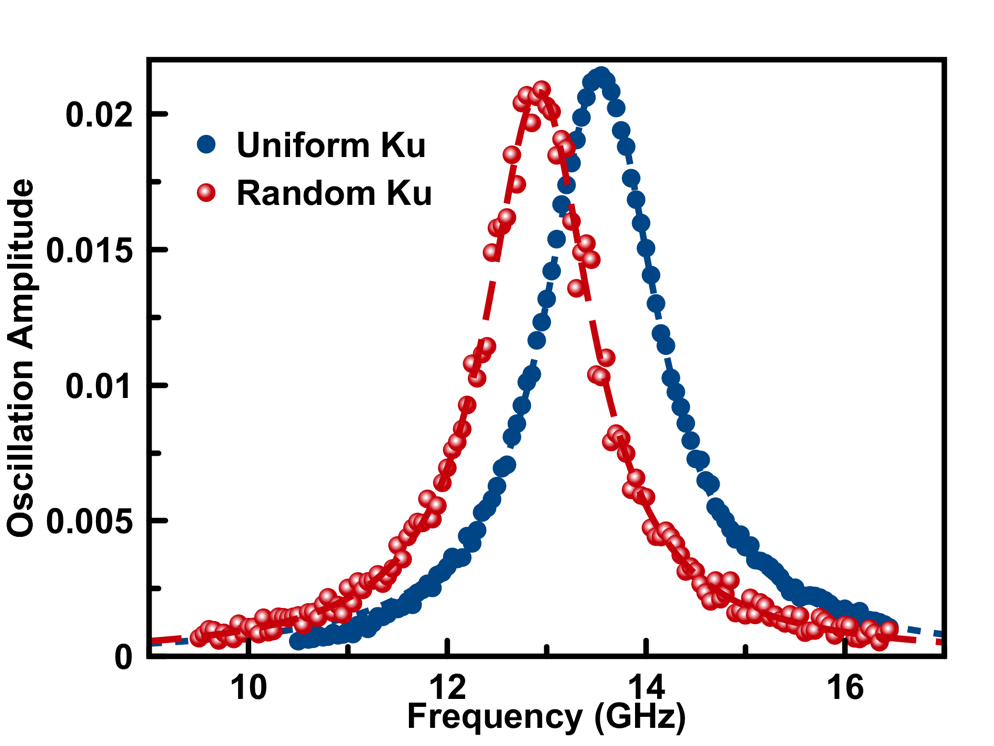
\includegraphics[width=50mm]{fig/CW_sim/random_spectrum.png}}
\subfigure{\label{fig:random_mode_profile}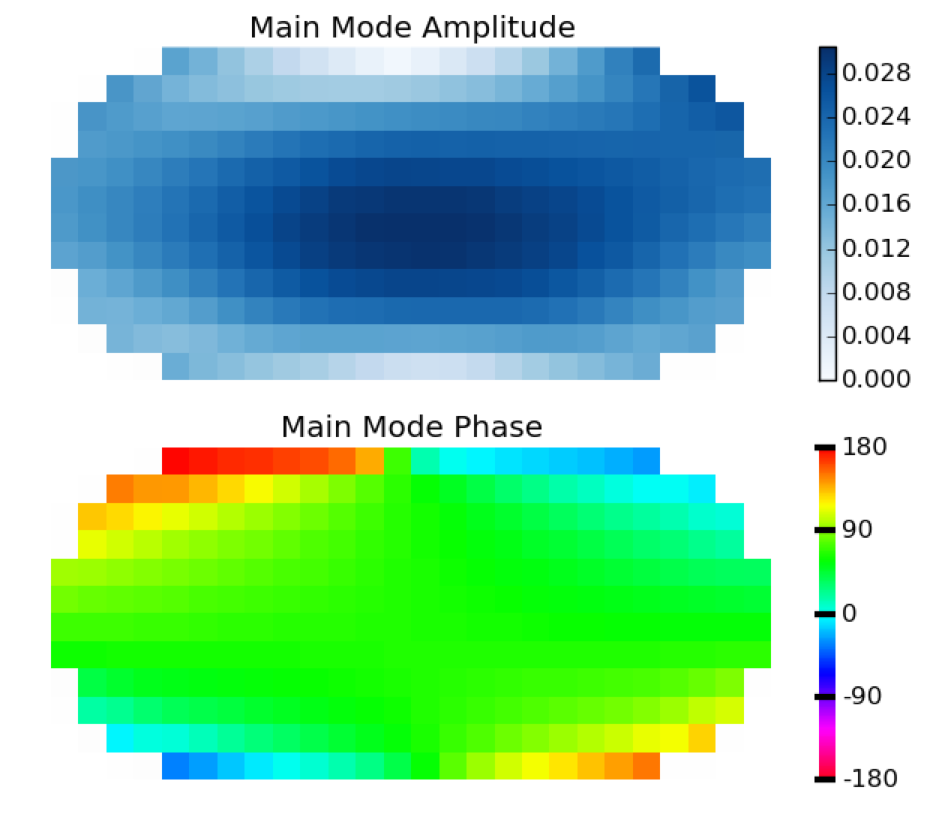
\includegraphics[width=50mm]{fig/CW_sim/mode_profile_2.png}}
\subfigure{\label{fig:Hk_dist}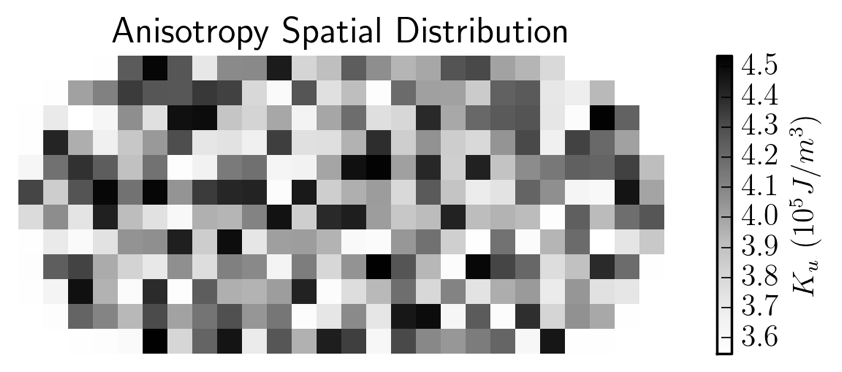
\includegraphics[width=50mm]{fig/CW_sim/Kudist.png}}
\caption{(a).Simulated spectrum with random magnetic anisotropy(in red dot) compared with spectrum with uniform magnetic anisotropy(blue dot) (b) Top: Spatial profile of the mode amplitude excited. Bottom: Spatial profile of the mode phase. (c)Spatial distributions of the magnetic anisotropy when introducing the random distributed magnetic anisotropy in OOMMF.}
\end{figure*}


In fact, since the CoFeB free layer is composed of grains, each with slightly different anisotropy, with strong exchange coupling inside of the grain and weaker exchange coupling among the grains\cite{grain}. In our simulation, by introducing random anisotropy field and decreasing the exchange stiffness with micromagnetic cell size close to the typical grain size of the CoFe crystals, we are reproducing the locally variant anisotropy field among the free layer, which contributes to the non-zero intercept $\Delta f_0$ we observed from previous ST-FMR measurement. Thus, we can qualitatively quantify the degree of random fluctuations of the magnetic anisotropy in the free layer of the MTJs.  



\begin{figure}[h!]
  \centering
  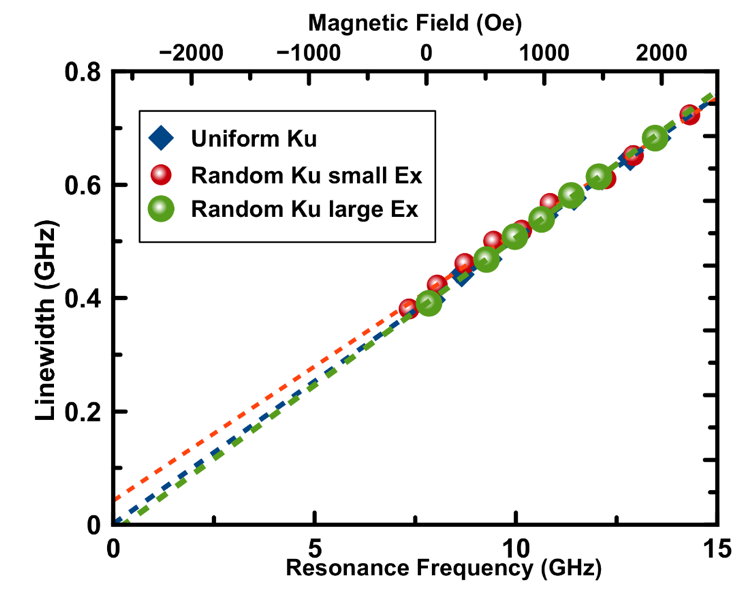
\includegraphics[width=0.8\textwidth]{fig/CW_sim/LW_summary.png}
  \caption{Summary of simulated linewidth plotted versus resonance frequency with different material parameters. From the plot only random magnetic anisotropy combined with small exchange stiffness leads to a significant linewidth intercept at zero resonance frequency.}
  \label{fig:CW_lw_summary}
\end{figure}


\begin{table}[h!]
\centering
 \begin{tabular}{||c c c||} 
 \hline
  & Gilbert damping $\alpha$  & Intercept $\Delta f_0$\\ [2.0ex] 
 \hline\hline
 Uniform
Uniform  & 0.05 & 0.0016$\pm$0.0064  \\ 
 \hline
 Random Ku with small Ex  & 0.047 & 0.043 $\pm$0.013 \\
 \hline
 Random Ku with large Ex  & 0.051 & -0.0027$\pm$0.0088  \\
 \hline
\end{tabular}
\caption{Table to test captions and labels}
\label{table:summary_LW}
\end{table}

We can summarize the simulation results from Table\ref{table:summary_LW}. It is clear that only combining low exchange stiffness with random fluctuations of magnetic anisotropy would lead to linewidth broadening at zero resonance frequency.

\newpage
\section{Micromagnetic Simulations}
In order to fully understand the magnetic dynamics being excited in the Magnetic Tunnel Junctions, we perform micromagnetic simulations using OOMMF package\cite{OOMMF}. To fully account for all magnetic interactions in the MTJ, we use a three dimensional model with three main functional layers: free layer, SAF top and SAF bottom layer. In the simulation, spin wave dynamics is excited by a combined pulse of ST and Oersted field, both resulting from a sinc-shaped spatially uniform current pulse with the amplitude $J_{C}\frac{\sin(2\pi f_{c} t^{'})}{2\pi f_{c}t^{'}} $ with the amplitude the cut-off frequency around 20 GHz, and the time variable $t_{0}$ 500 ps. The need to combine the excitation from Spin torque and Oersted field is to include the uniform and non-uniform spin wave modes in the MTJs\cite{Modes}.
The spatial profile of the Oersted field is assumed to be that of a long wire with elliptical cross section. The direction of the ST vector acting on the free layer is determined by the magnetization orientation of the SAF top layer.Spectrum of spin wave eigenmodes is obtained via the Fast-Fourier-transform (FFT) of the time dependent in-plane component of the MTJ net magnetic moment. 




\begin{figure}[!ht]
\centering
\subfigure{\label{fig:MR18}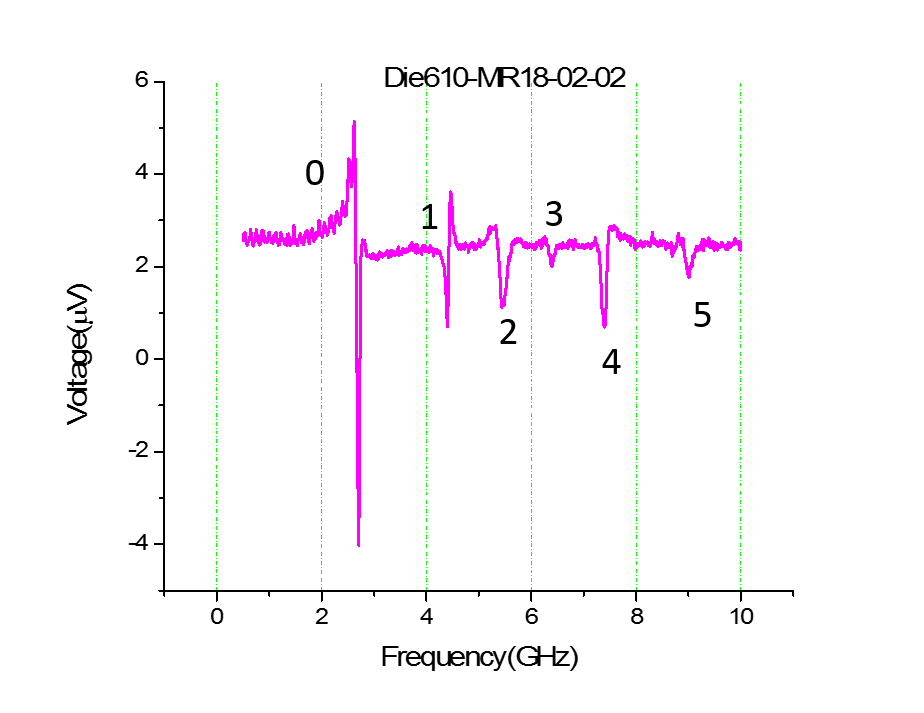
\includegraphics[width=75mm]{fig/MR18.png}}
\subfigure{\label{fig:Simulation}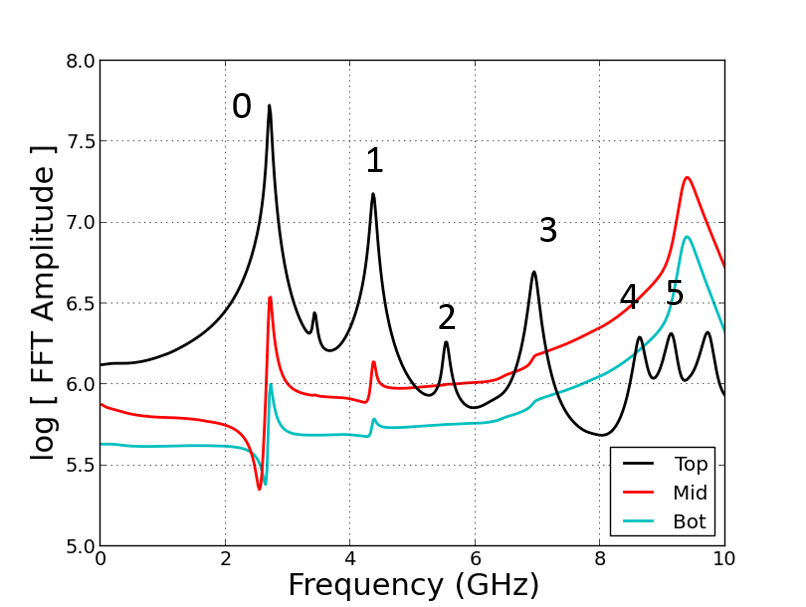
\includegraphics[width=75mm]{fig/simulation.png}}
\caption{(a) ST-FMR spectrum of a 30 nm by 150 nm stadium-shaped STT-MRAM element. Several spin wave eignemode resonances are seen in the spectrum. (b)Fitted spectrum from micromagnetic simluations.}
\end{figure}

Fig.\ref{fig:MR18} shows a typical ST-FMR spectrum from our measurement. For this sample, we can identify five spin wave modes. The zero mode is the uniform excitation and we have already used this mode to fit for magnetic anisotropy and Gilbert damping value. The other four modes are non-uniform modes excited along the edges. On the left, Fig.\ref{fig:Simulation} shows the simulated spectrum from our micromagnetic calculations. As we discussed before, we perform the Fast-Fourier-transform on the in-plane component of the MTJ net magnetic moment and plot it against driven frequency. The top layer is the free layer and the middle(bottom) is the SAFTop(SAFBottom) layer. As we can see from the plot, the amplitude of the top layer is definitely much larger than the other layers, meaning the excitation of the MTJs is dominant by the free layer. The peaks in the spectrum are corresponding to the spin wave modes we observe from the experiment. By tuning the material parameter such as magnetic anisotropy and exchange constant, we can match the frequency position of the first zero mode and the second mode. So firstly, from micromagnetic simulations, we can determine the magnetic anisotropy to be $3.13*10^5 J/m^3$ and exchange stiffness constant to be around $5*10^{-12} J/m$.

Next we would like to understand the nature of the modes we excited. To do this, we perform the spatial mapping of the mode amplitude and plot it in Fig.\ref{fig:mode}. Starting from the top left, we list the model profile for all the five modes. As expected, the first mode is uniform excitation so the amplitude of this mode is uniform. The second mode has two nodes along the short axis. So we label it as Mode(2,0). Then we have modes from Mode(3,0) and Mode(4,0) which have three or four nodes along the short axis. The last mode has one node along the long axis, so it is labeled as Mode(0,1).





\begin{figure}[h!]
  \centering
  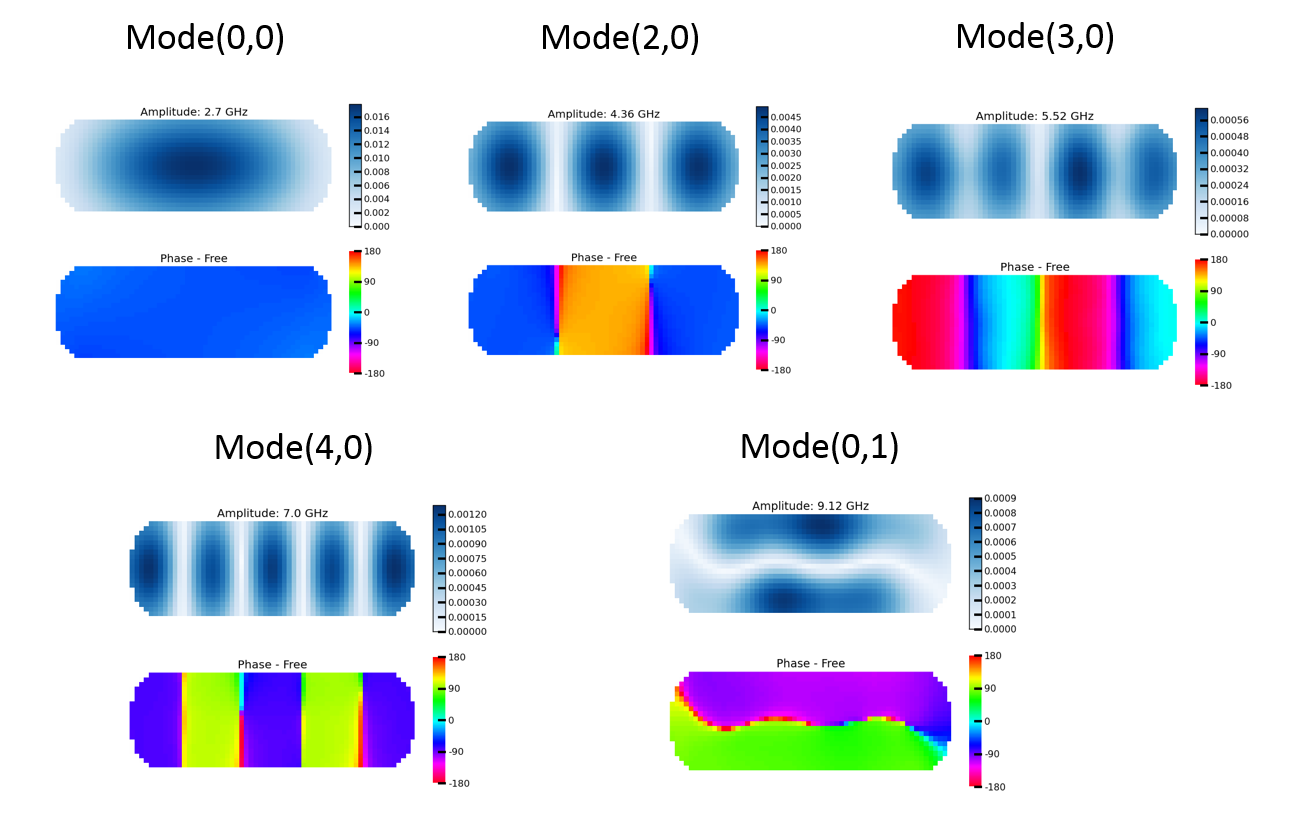
\includegraphics[width=1.0\textwidth]{fig/Mode_pic.png}
   \caption{Spatial mapping of modes excited in the micromagnetic simulations. }
  \label{fig:mode}
\end{figure}

After that, we find that no matter how we tune the magnetic anisotropy and exchange constant, the latter three modes can not be matched very well from experiment and simulations. So we have to consider another possibilities. One thing to consider is magnetic edge damage of the MTJ element. Such modifications are unavoidable in the STT-MRAM fabrication process due to etching of the element, and they are predicted to have significant impact on current-driven switching of the free layer. We tested several micromagnetic models of the magnetic edge damage and found how these models modify the frequencies of spin wave eignemodes. We then compared the  model’s predictions to our measurments of spin wave spectra by spin torque ferromagnetic resonance. This comparison allowed us to determine which model best describes the experimental data. More specifically, we have tested three models of the magnetic edge damage: 

-	Magnetic dilution model. In this model, saturation magnetization and exchange stiffness of the free layer of STT-MRAM are reduced in the edge region.
-	STT-MRAM shape distortion model. In this model, the MTJ nanopillar shape is distorted with respect to its nominal shape.
-	Anisotropy reduction model. In this model, magnetic shape anisotropy is reduced near the sample edges.

Fig.\ref{fig:edge_damage} shows the results by exploiting edge damage model in the simulation. From this plot we find that this mode cannot adequately describe the experimentally observed spectrum of spin wave eignemodes in STT-MRAM samples we experimentally studied. Compared with the edge anisotropy model in Fig.\ref{fig:edge_ani}, now we have a much better agreement between experiment and simulations. We, therefore, conclude that the major impact of the STT-MRAM edge on magnetic properties of the device is reduction of perpendicular magnetic anisotropy near the device edge. This reduction can result in nucleation of current-driven magnetization reversal near the sample edges  Comparison of ST-FMR measurements of spin wave mode frequencies can quantify the degree of magnetic anisotropy reduction near the sample edges. We discuss how this can be accomplished in the next paragraph. 

\begin{figure}[!ht]
\centering
\subfigure{\label{fig:edge_damage}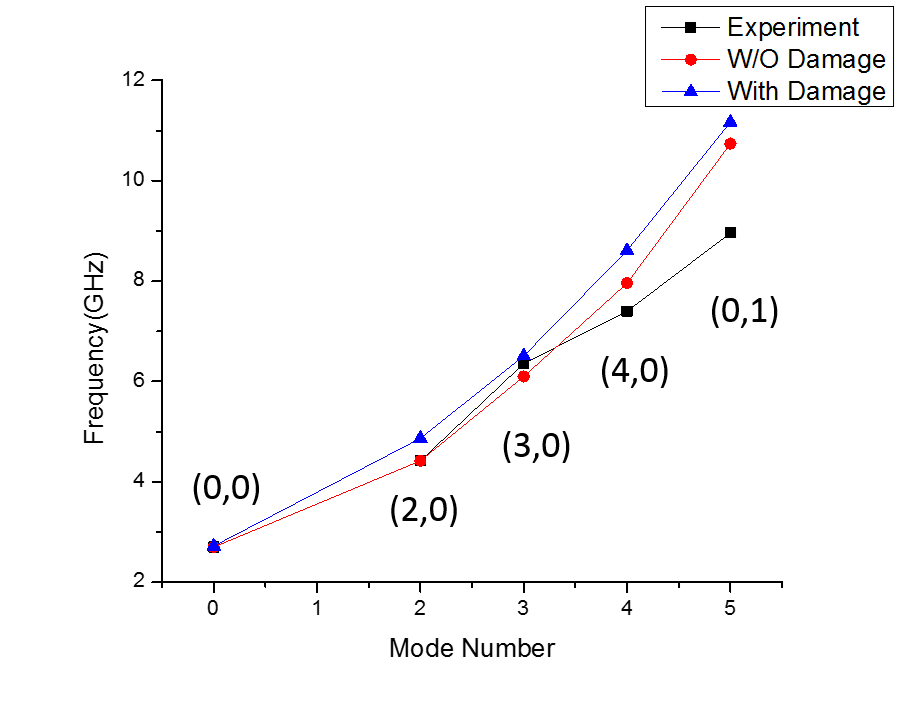
\includegraphics[width=80mm]{fig/edge_damage.png}}
\subfigure{\label{fig:edge_ani}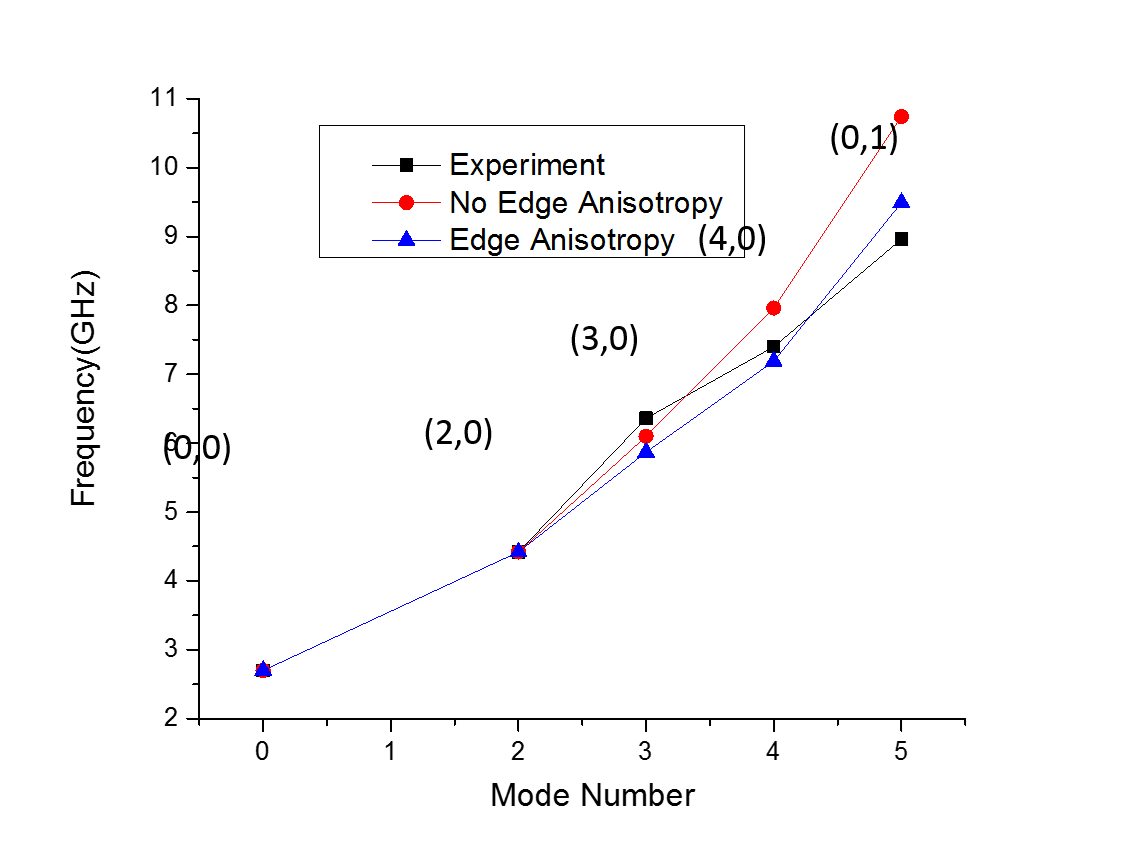
\includegraphics[width=80mm]{fig/edge_ani.png}}
\caption{(a) ST-FMR spectrum of a 30 nm by 150 nm stadium-shaped STT-MRAM element. Several spin wave eignemode resonances are seen in the spectrum. (b)Fitted spectrum from micromagnetic simluations.}
\end{figure}

From fitting the first and second mode frequencies, we already have a confidence value of magnetic anisotropy and exchange constant. Then we employ the models of spatially non-uniform parameters of the free layer. The blue symbols in the left panel of Fig.\ref{fig:edge_damage} show results of the simulations for the magnetic edge dilution model. In this model, both the saturation magnetization and the exchange constant of the free layer are gradually reduced from their bulk values to zero at the free layer edge. The distance over which this reduction takes place was chosen to be in the 2.5 nm to 7.5 nm range (typical material damage depths due to various types of etching). It is clear from Fig.\ref{fig:edge_damage} that the magnetic dilution model does not improve the agreement between theory and experiment. We have also found that shape distortions of the free layer do not reproduce the experimental results well. In contrast, reduction of magnetic anisotropy from  $3.13*10^5 J/m^3$ in the free layer interior to $3.03*10^5 J/m^3$ at the free layer edge over a distance of 2.5 nm gives a much better agreement with the experimental data as shown by blue symbols in the Fig.\ref{fig:edge_ani}. This type of fitting allows us to obtain the exchange stiffness constant of the free layer, its perpendicular magnetic anisotropy value and the magnitude of reduction of the perpendicular anisotropy at the sample edge.















\section{Circular STT-MRAM Devices with Broken Symmetry}

While stadium-shaped or rectangular samples are convenient for studies of the edge damage due to their particularly simple spin mode structure, studies of circular STT-MRAM samples are important because this shape is the primary candidate for STT-MRAM. We performed ST-FMR measurements of circular STT-MRAM samples and measured their spin wave spectra as a function of the nanopillar diameter. Fig.\ref{fig:circularmode} shows two examples of such spectra for STT-MRAM cells with diameters of 250 nm and 80 nm measured as a function of out-of-plane magnetic field. A large number of modes are observed for the 250 nm sample due to the relatively weak geometric confinement of spin waves in the large structure. For these larger devices, it would be relatively hard to identify all the modes excited. While you can still fit for some of the spin-wave modes, the frequency spacings between each mode is relatively small, which makes further quantitatively analysis.
 
 \begin{figure}[h!]
  \centering
  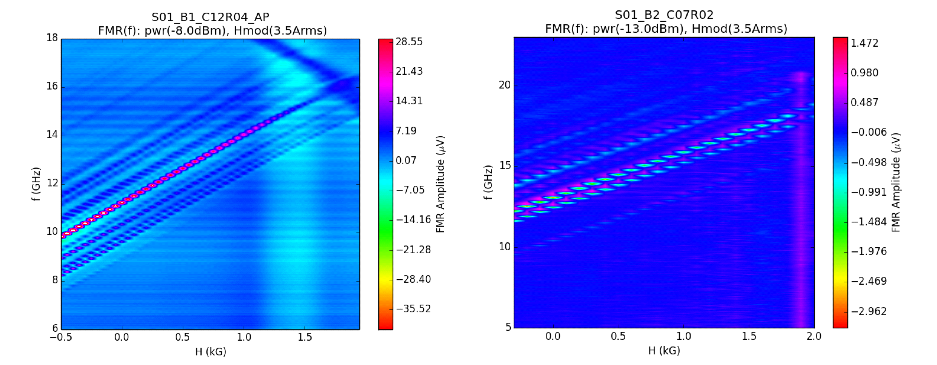
\includegraphics[width=1\textwidth]{fig/FieldMod/ap-p.png}
   \caption{ST-FMR spectra of circular STT-MRAM cells with 250 nm diameter (left) and 80 nm diameter (right) measured as a function of the out-of-plane magnetic field applied to the nanopillar.}
  \label{fig:apandp}
\end{figure}

When we move to much smaller devices, fewer spin wave modes with larger inter-mode frequency gaps are seen for the 80 nm sample. The spin wave mode structure in circular STT-MRAM samples is qualitatively different from that in the stadium-shaped samples. The modes are characterized by two indexes: n = (0, 1, 2…) and L = (0,1)\cite{excitation2}. The index n gives the number of spin wave nodes in the radial direction, while the index L describes azimuthal phase variation of the mode. Spatial profiles of the three lowest-frequency modes in a perfectly circular sample with 60 nm diameter are shown in Fig. \ref{fig:circularmode}. The first mode(labelled as (0,0)) is the lowest-frequency quasi-uniform mode. The second mode(labelled as (0,1)) is the first higher-order mode, it has larger amplitude at the edges and a node at the center. The last mode in \ref{fig:circularmode} is labelled as (1,0), which has a node along the edges of the device. This is the case when we have a perfect circular shape MRAM sample.
 
\begin{figure}[h!]
  \centering
  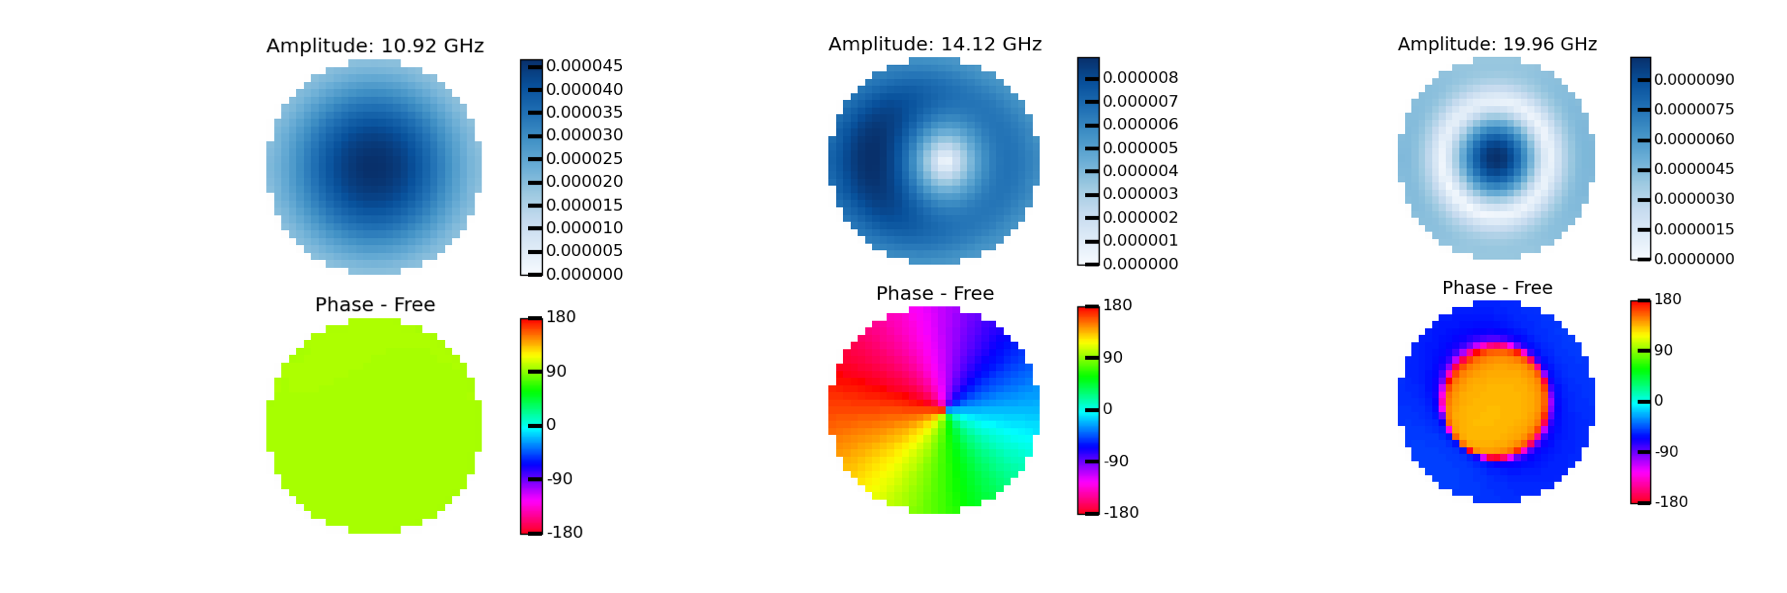
\includegraphics[width=0.8\textwidth]{fig/FieldMod/mode-profile.png}
   \caption{Three lowest-frequency spin wave eigenmodes of the free layer of a circular STT-MRAM sample with 60 nm diameter. The top image shows the spatial map of the amplitude of the mode while the bottom image shows the spatial map of the spin wave mode’s phase}
  \label{fig:circularmode}
\end{figure}


However, in our experimental data, we find the frequency of the second higher-order mode(label as mode(0,1)) is considerably larger than micromagnetic simulations. To  confirm this finding, we measured more than ten MRAM devices with the same nominal dimension. The ST-FMR spectra of all circular samples we studied exhibit one common feature: the lowest frequency (quasi-uniform) mode always appears as a singlet while the two higher frequency modes appear as a doublet with relatively small inter-mode frequency splitting (~ 1GHz). Furthermore, we find there is a distribution of all the three modes frequencies. Fig.\ref{fig:stat1} summarizes the experimental results, which shows the statistics of the mode frequencies at zero field for different modes. We find that the distribution is somewhat skewed towards lower frequencies. We also notice that there is a clear visibly larger spread for the (1,0) and (0,1) modes compared to the (0,0) mode. This is because the (1,0) and (0,1) mode frequencies are also affected by random in-plane anisotropy fluctuations due to e.g. elliptical shape distortions.


\begin{figure*}[h!]
\centering     
\subfigure{\label{fig:stat1}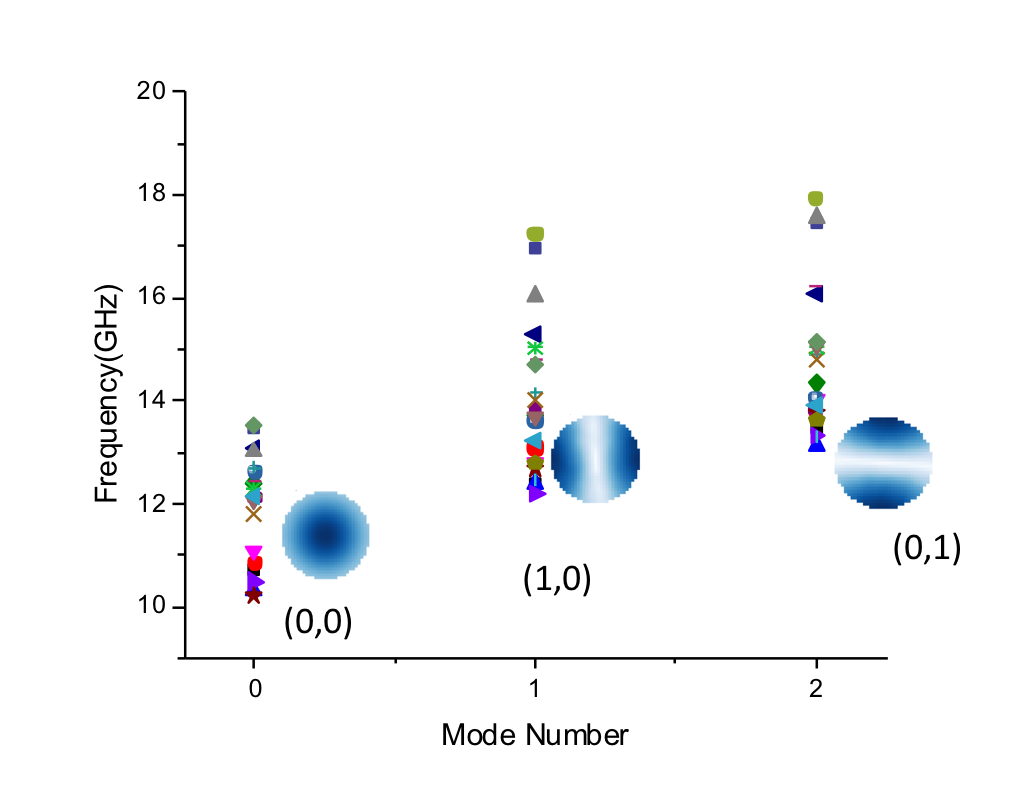
\includegraphics[width=80mm]{fig/broken/stastic-1.png}}
\subfigure{\label{fig:stat2}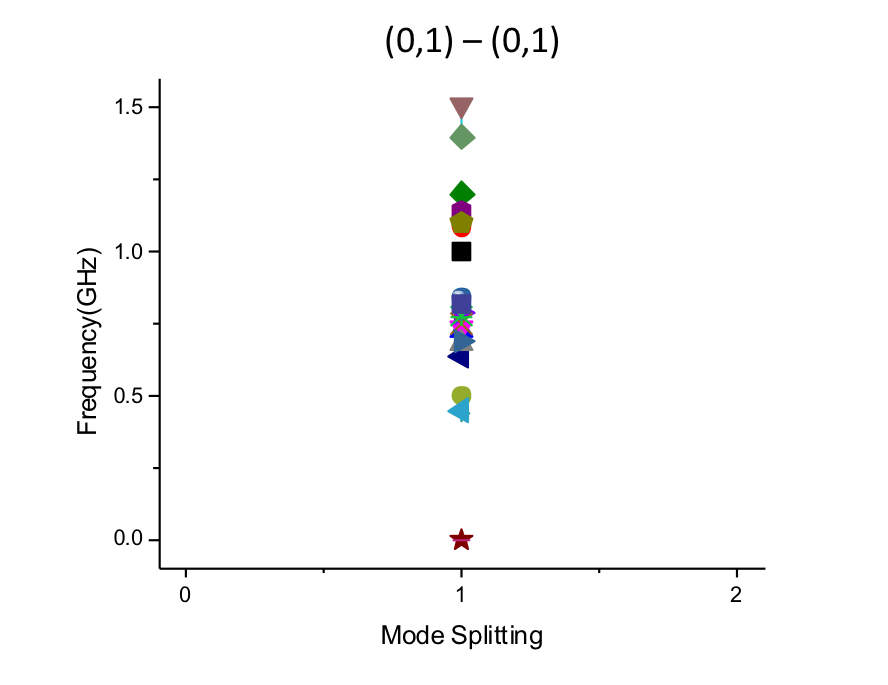
\includegraphics[width=80mm]{fig/broken/stastic-2.png}}
\caption{(a) Statistics of the mode frequencies at zero field for different modes. (b) Statistics of mode splitting between the (1,0) and (0,1) modes for 80 nm samples.
}
\end{figure*}


\begin{figure*}[h!]
\centering     
\subfigure{\label{fig:freq10}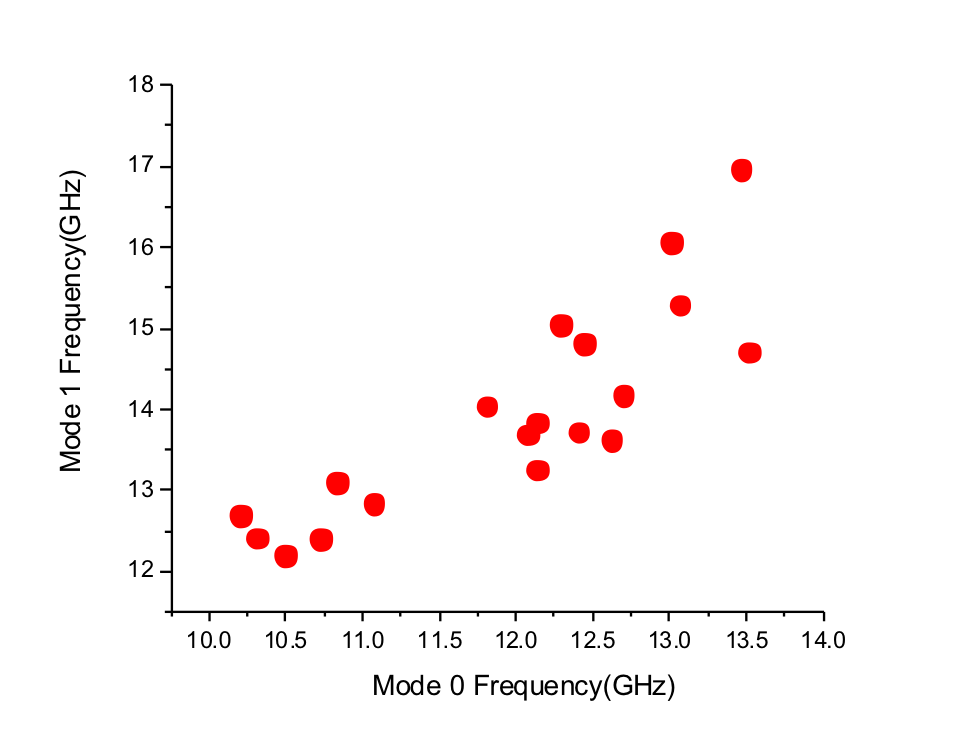
\includegraphics[width=80mm]{fig/broken/freq1-0.png}}
\subfigure{\label{fig:freq20}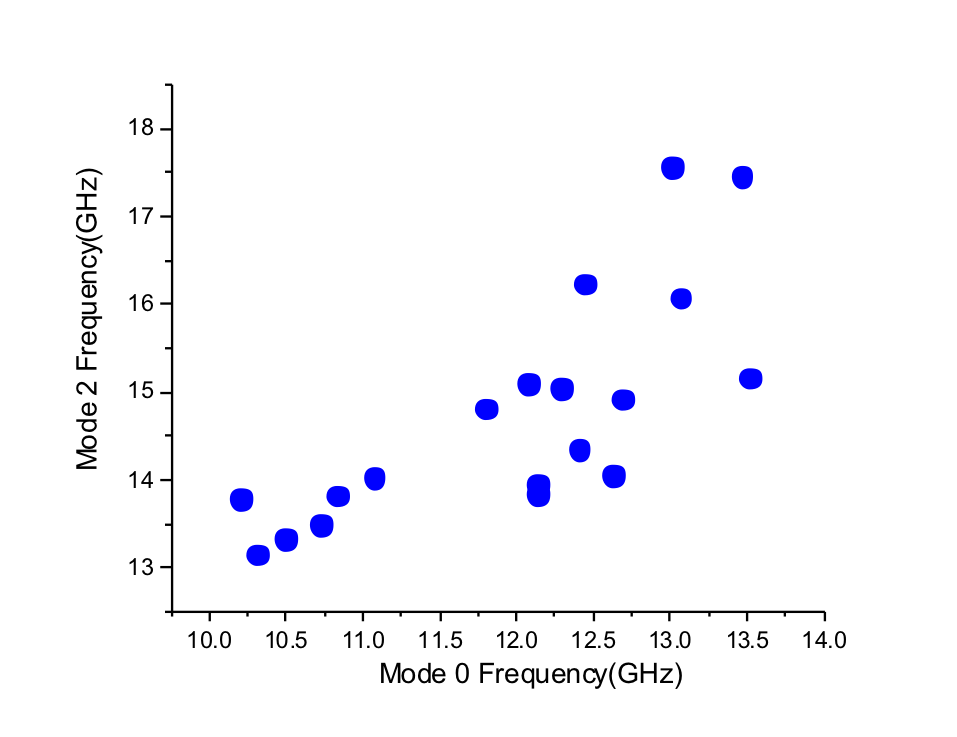
\includegraphics[width=80mm]{fig/broken/freq2-0.png}}
\caption{Statistics of mode splitting for 80 nm sample. (a):Frequency of the Mode 1 versus frequency of the Mode 0. (b):Frequency of the Mode 2 versus frequency of the Mode 0}
\end{figure*}



The (0,0) mode frequencies can be used to quantify the average anisotropy field and the anisotropy field distribution. It is also interesting to compare the distributions of the main modes as a function of the device dimensions. Fig.\ref{fig:freq10} shows the frequency of the Mode 1 versus frequency of the Mode 0 and Fig.\ref{fig:freq20} shows the frequency of the Mode 2 versus frequency of the Mode 0. We can find a clear linear correlation between the quasi-uniform and the higher order mode frequencies, which reveals sample-to-sample perpendicular anisotropy fluctuations but fairly sample-independent exchange energy of the free layer. Since the exchange energy is closely related with sample dimensions, this also shows that the device geometries do not have large variations.


As we mentioned earlier, micromagnetic simulations of circular devices do not match with experimental data. Fig.\ref{fig:exp_spectrum} ST-FMR spectrum of spin wave eignemodes in a circular 60 nm diameter MTJ nanopillar measured at 1 kG out-of-plane field. There are five modes are visible at low frequency and we are concentrating on the lowest three spin-wave modes. Fig.\ref{fig:spectrum_60} shows a simulated spectrum for a 60 nm STT-MRAM element. Vertical dashed lines indicate measured mode positions. Experimentally the frequency spacing between mode 1 and mode 2 is less than 1 GHz. However, the spacing in the micromagnetic simulations is quite large.


\begin{figure*}[h!]
\centering     
\subfigure{\label{fig:exp_spectrum}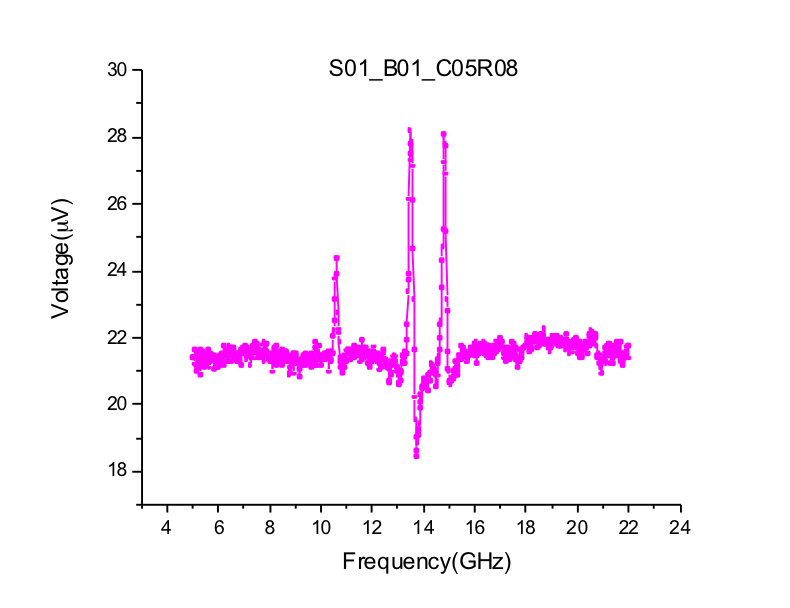
\includegraphics[width=80mm]{fig/broken/exp_spectrum.png}}
\subfigure{\label{fig:spectrum_60}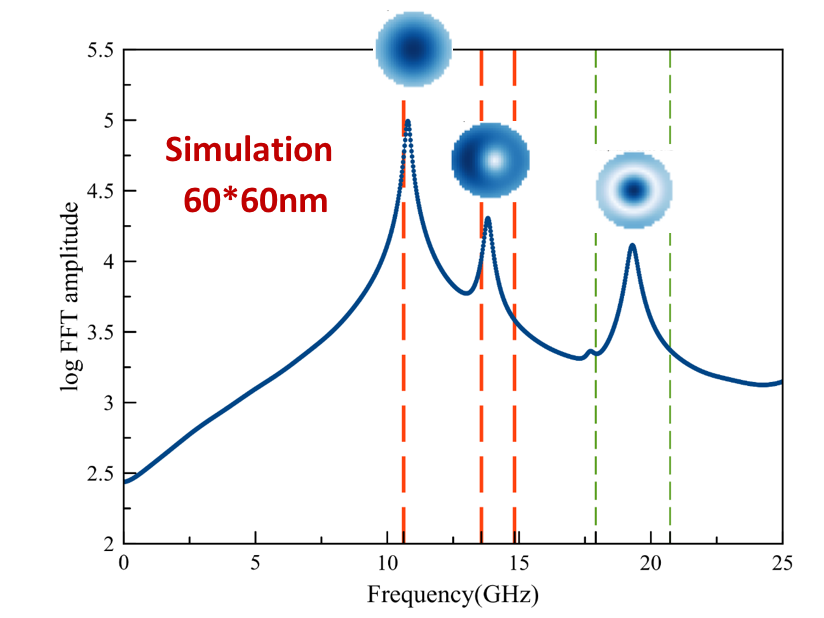
\includegraphics[width=80mm]{fig/broken/spec_60nm.png}}
\caption{(a) ST-FMR spectrum of spin wave eignemodes in a circular 60 nm diameter MTJ nanopillar measured at 1 kG out-of-plane field. (b)Simulated ST-FMR spectrum of a 60 nm circular STT-MRAM element. Vertical dashed lines indicate measured mode positions. Micromagnetic simulated mode profiles are shown next to each mode.}
\end{figure*}


The mode structures and discrepancy can be explained if the perfect circular symmetry of the system is broken. There are several candidates for this broken symmetry and the most possible one is the elliptical distortion of the nanopillar shape. During the fabrication of the STT-MRAM elements, certain processes, such as edge etching, are prone to cause device actual dimension to deviate from perfect circular shape.Such symmetry breaking has little effect on the quasi-uniform (n=0,L=0) mode, but it splits the (n=0,L=1) mode into two modes with a single node along either the short or the long axis of the ellipse. We then examine the effect of the shape distortion on the excited spin wave mode structure via micromagnetic simulations.  In the simulations, we replace the perfect circular shape by an ellipse with varying eccentricity. By varying eccentricity, we influence the degree of the spin wave mode splitting. Fig.\ref{fig:spectrum_68_52} shows a spectrum with device dimension 68 nm * 52 nm. The mode (0,1) split into two modes as we expect. Fig.\ref{fig:spectrum_64_56} shows a spectrum with device dimension 64 nm * 56 nm. As we can compare between those two spectrums, the first-order mode splits into two modes and the frequency gap between those two modes is increasing with increased eccentricity. For devices with larger eccentricity the mode gap is larger, which indicates the mode gap is closely related with shape deviations from perfect circular.

\begin{figure*}[h!]
\centering     
\subfigure{\label{fig:spectrum_64_56}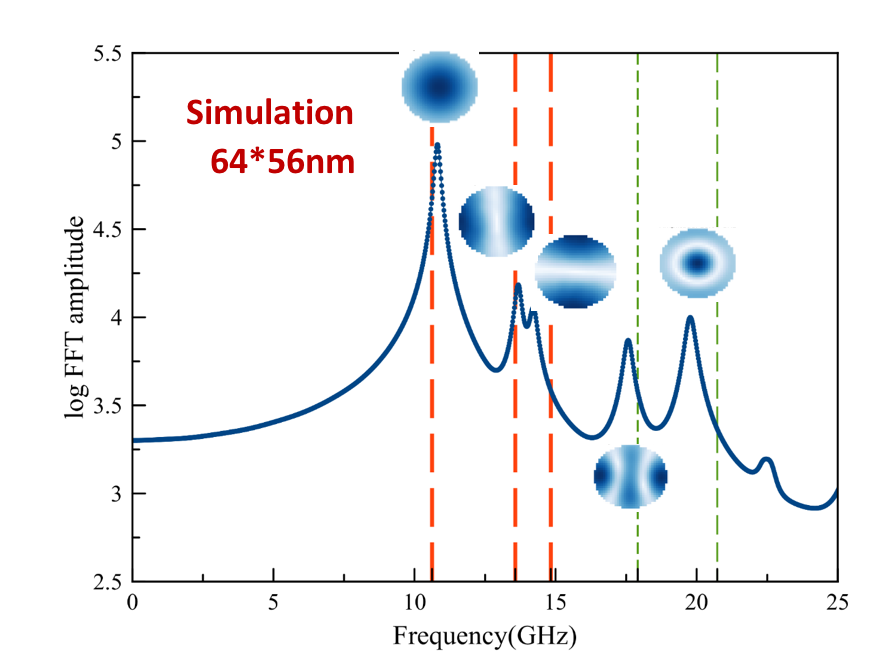
\includegraphics[width=50mm]{fig/broken/spec_64_56nm.png}}
\subfigure{\label{fig:spectrum_68_52}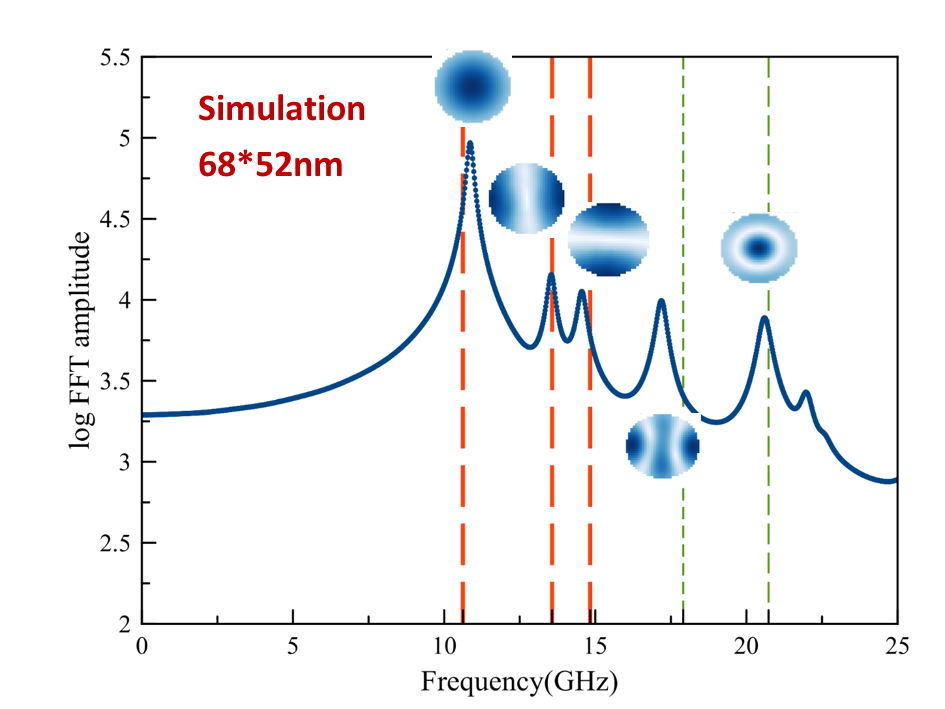
\includegraphics[width=50mm]{fig/broken/spec_68_52nm.png}}
\subfigure{\label{fig:eccentricity}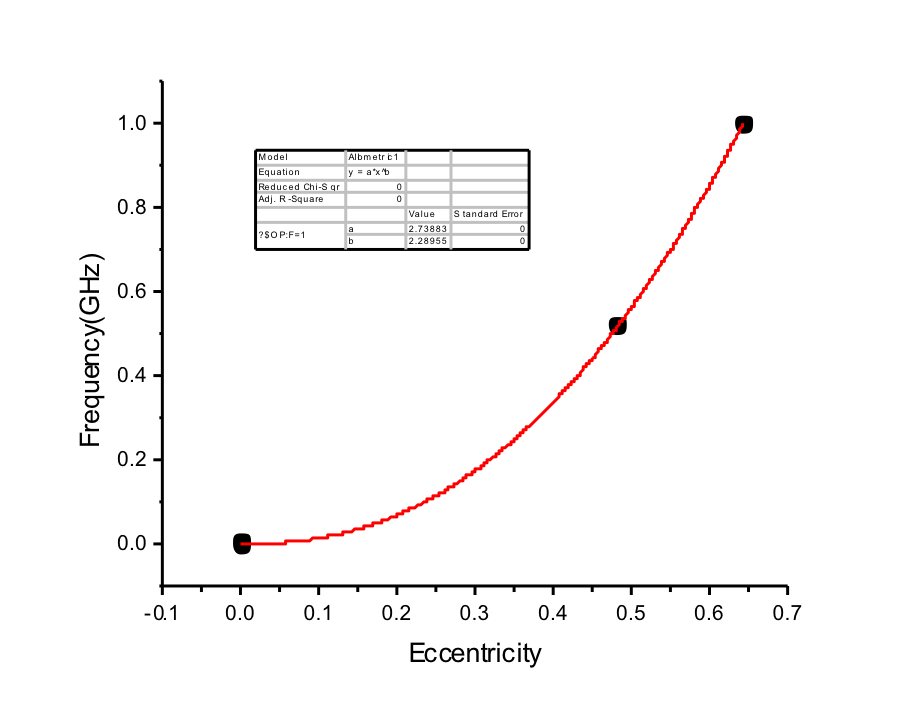
\includegraphics[width=50mm]{fig/broken/ecc.png}}
\caption{ST-FMR spectrum of spin wave eignemodes in a circular 60 nm diameter MTJ nanopillar measured at 1 kG out-of-plane field. Five modes are visible at low frequency. (b)Simulated ST-FMR spectrum of a 5268 nm2 elliptical STT-MRAM element. Vertical dashed lines indicate measured mode positions. Micromagnetic simulated mode profiles are shown next to each mode.  (right) Simulated splitting (frequency gap) of (n=0,L=+1) mode plotted versus eccentricity}
\end{figure*}


With that in mind, Fig.\ref{fig:spectrum_64_56} shows the best micromagnetic fit to the experimental spectrum for a circular 60 nm MTJ nanopillar shown in Fig.\ref{fig:exp_spectrum}. The vertical dashed lines indicate the measured mode frequencies. The simulated mode frequencies agree well with the experimental results suggesting that the mode splitting observed in the experiment arises from MTJ shape distortions. The micromagnetic fitting gives the value of the perpendicular anisotropy (Ku = $4.3*10^5 J/m^3 $) and exchange stiffness constant (A = $6.01*10^{-12}$ J/m) of the free layer.  Furthermore, Fig.\ref{fig:eccentricity} shows simulated splitting (frequency gap) of (n=0,L=+1) mode plotted versus eccentricity. This enables us to establish a correlation between the measured frequency gap and the degree of shape distortion, which is difficult to measure directly.






\begin{figure}[h!]
  \centering
  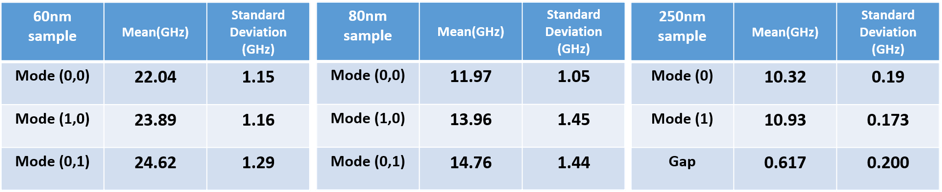
\includegraphics[width=0.8\textwidth]{fig/broken/stastic-mode.png}
   \caption{Three lowest-frequency spin wave eigenmodes of the free layer of a circular STT-MRAM sample with 60 nm diameter. The top image shows the spatial map of the amplitude of the mode while the bottom image shows the spatial map of the spin wave mode’s phase}
  \label{fig:statmod1}
\end{figure}


We then study the mode splitting as a function of the nanopillar diameter. More than 15 devices of each MTJ diameter were measured to obtain reliable statistical distributions of the mode frequencies.  First, we find that the 250 nm devices do not show splitting of the (n=0,L=+1) mode. This supports the picture of splitting of this mode due to deviations from the perfectly circular shape (little process-induced ellipticity is expected for these large circular devices). Second, for the larger 250 nm devices, standard deviation of the frequency distribution is much smaller than that for the 60 nm and 80 nm devices. We can then conclude that low-energy mode frequencies are sensitive to the average anisotropy over the free layer area. In the larger devices, averaging over a larger number of crystallographic grains and results in a tighter distribution of the free layer anisotropy values.







\newpage

\section{Possible Origin of WER Correlation with ST-FMR}

We also collected preliminary data suggesting a correlation between ST-FMR spectra of circular MTJ nanopillars with write error rates of the devices.  Fig.\ref{fig:WERSTFMR} shows ST-FMR spectrum of spin wave eignemodes in a circular 40 nm diameter MTJ nanopillar as a function of out-of-plane magnetic field. This sample shows anomalous WER behavior (ballooning).

\begin{figure}[h!]
  \centering
  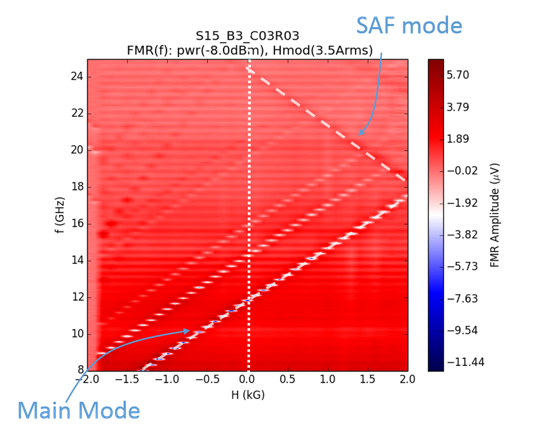
\includegraphics[width=0.6\textwidth]{fig/FieldMod/FMR-WER.png}
   \caption{ST-FMR spectrum of spin wave eignemodes in a circular 40 nm diameter MTJ nanopillar with known anomalous WER behavior measured as a function of out-of-plane magnetic field. The SAF spin wave mode and the quasi-uniform free layer mode are labeled by dashed lines in the figure.}
  \label{fig:WERSTFMR}
\end{figure}


For this device, the frequency of the SAF mode in zero field is nearly twice the resonance frequency of the quasi-uniform mode of the free layer. This frequency coincidence condition suggests that a nonlinear three-magnon process (confluence of two magnons of the quasi-uniform mode into a single SAF mode magnon) should be resonant for this device in zero field. Such non-linear resonant scattering channel can drain energy an angular momentum supplied by spin torque t the free layer and impede the free layer switching process. Therefore, this nonlinear scattering process is suspected origin of the anomalous WER behavior. For all devices studied so far, we find that MTJs exhibiting anomalous WER do satisfy this nonlinear resonant scattering (frequency coincidence) condition, while all devices with normal WER do not satisfy the nonlinear resonant scattering condition